% Paper: compositional self-improvement, checks before training.
% Build: make (tectonic) or make latexmk. Numbers, tables and figures in
% generated/ come from `uv run python -m gainpred.writeup` and are never edited
% by hand. Source lines are kept to 80 characters: `make wrap` (PDF unchanged).
\documentclass{article}

% NeurIPS style in preprint mode. The 2026 style file was not yet published at
% media.neurips.cc (15 Nov 2026), so the 2025 one is used; swap the file and
% this line.
\usepackage[preprint]{neurips_2025}

\usepackage[utf8]{inputenc}
\usepackage[T1]{fontenc}
\usepackage{xr-hyper}       % references into supplement.tex (prefix S-)
\usepackage{hyperref}
\usepackage{url}
\usepackage{booktabs}
\usepackage{amsfonts}
\usepackage{amsmath}
\usepackage{amsthm}
\usepackage{nicefrac}
\usepackage{microtype}
\usepackage{xcolor}
\usepackage{graphicx}
\usepackage{amssymb}
\usepackage{array}
\usepackage{float}             % [H] placement for tables and figures
\usepackage{tikz}
\usetikzlibrary{arrows.meta,positioning,calc}
\usepackage[section,above,below]{placeins}
\usepackage[title]{appendix}   % headings read "Appendix A ..."
% Generated by `uv run python -m gainpred.writeup`; do not edit by hand.
% Numbers cited in the text of section 4, so the prose cannot drift from the
% data.
% Marked 'after': computed after the evaluation runs (not part of the frozen
% analysis).
\newcommand{\gpCases}{258}
\newcommand{\gpCorrect}{249}
\newcommand{\gpCorrectPct}{96.5}
\newcommand{\gpCasesAll}{270}
\newcommand{\gpNoOutcome}{12}
\newcommand{\gpCorrectAllPct}{92.2}
\newcommand{\gpCorrectModelTwo}{84}
\newcommand{\gpCasesModelTwo}{86}
\newcommand{\gpCorrectModelThree}{82}
\newcommand{\gpCasesModelThree}{86}
\newcommand{\gpCorrectModelFour}{83}
\newcommand{\gpCasesModelFour}{86}
\newcommand{\gpHarmful}{43}
\newcommand{\gpDidHarm}{15}
\newcommand{\gpTaughtWrong}{28}
\newcommand{\gpByBasics}{10}
\newcommand{\gpByBasicsCorrect}{1}
\newcommand{\gpByNovelty}{175}
\newcommand{\gpByNoveltyCorrect}{175}
\newcommand{\gpByAgreement}{73}
\newcommand{\gpByAgreementCorrect}{73}
\newcommand{\gpByMinKept}{6}
\newcommand{\gpCorrectNoBasics}{255}  % after
\newcommand{\gpCorrectNoBasicsPct}{98.8}  % after
\newcommand{\gpOursCorrect}{249}
\newcommand{\gpOursCorrectPct}{96.5}
\newcommand{\gpOursHarmFlagged}{43}
\newcommand{\gpOursWeakCorrect}{1}
\newcommand{\gpBaselineCorrect}{224}
\newcommand{\gpBaselineCorrectPct}{86.8}
\newcommand{\gpBaselineHarmFlagged}{38}
\newcommand{\gpBaselineWeakCorrect}{4}
\newcommand{\gpVariantCorrect}{242}  % after
\newcommand{\gpVariantCorrectPct}{93.8}  % after
\newcommand{\gpVariantHarmFlagged}{33}  % after
\newcommand{\gpVariantWeakCorrect}{6}  % after
\newcommand{\gpWeakCases}{10}
\newcommand{\gpBaselineCostPct}{56}
\newcommand{\gpChecksCostPct}{9}
\newcommand{\gpNoveltyLevel}{50}
\newcommand{\gpConfirmedLevel}{38}
\newcommand{\gpNoveltyMarginLow}{40.2}  % after
\newcommand{\gpNoveltyMarginHigh}{60.9}  % after
\newcommand{\gpConfirmedMarginLow}{27.8}  % after
\newcommand{\gpConfirmedHarmCases}{42}  % after
\newcommand{\gpConfirmedMarginHigh}{50.7}  % after
\newcommand{\gpConfirmedPaysCases}{31}  % after
\newcommand{\gpRiseNothingUnderTwo}{25}
\newcommand{\gpRoundsCorrect}{52}  % after
\newcommand{\gpRounds}{57}  % after
\newcommand{\gpCtrlAfterSevenCorrect}{23.7}  % after
\newcommand{\gpCtrlAfterSevenLengthSix}{74.5}  % after
\newcommand{\gpCtrlAfterSevenPickLonger}{0.0}  % after
\newcommand{\gpWithheldSevenCorrect}{0.0}  % after
\newcommand{\gpWithheldSevenLengthSix}{99.6}  % after
\newcommand{\gpWithheldSevenPickLonger}{0.0}  % after
\newcommand{\gpEdgesFiveCorrect}{44.0}  % after
\newcommand{\gpEdgesFiveLengthSix}{0.0}  % after
\newcommand{\gpEdgesFivePickLonger}{27.7}  % after
  % numbers cited in the text (gainpred.writeup)
% Generated by `uv run python -m gainpred.floors_paper`; do not edit by hand.
% Numbers of the pilot on building on self-taught pieces and of its control
% (amendment 27);
% read after the runs from results/pilot/runs/. Not part of numbers.tex.
\newcommand{\gpClimbAgrFloorTwoLearned}{3}
\newcommand{\gpClimbAgrFloorTwoLowest}{99.9}
\newcommand{\gpClimbAgrFloorTwoDrop}{0.1}
\newcommand{\gpClimbAgrFloorTwoKeptRight}{99.9}
\newcommand{\gpClimbAgrFloorThreeLearned}{3}
\newcommand{\gpClimbAgrFloorThreeLowest}{99.9}
\newcommand{\gpClimbAgrFloorThreeDrop}{0.0}
\newcommand{\gpClimbAgrFloorThreeKeptRight}{100.0}
\newcommand{\gpClimbAgrFloorFourLearned}{3}
\newcommand{\gpClimbAgrFloorFourLowest}{99.9}
\newcommand{\gpClimbAgrFloorFourDrop}{0.1}
\newcommand{\gpClimbAgrFloorFourKeptRight}{100.0}
\newcommand{\gpClimbKeyFloorTwoLearned}{2}
\newcommand{\gpClimbKeyFloorTwoLowest}{100.0}
\newcommand{\gpClimbKeyFloorTwoDrop}{0.0}
\newcommand{\gpClimbKeyFloorTwoKeptRight}{100.0}
\newcommand{\gpClimbDirectFloorTwoLearned}{0}
\newcommand{\gpClimbDirectFloorTwoLowest}{0.0}
\newcommand{\gpClimbDirectFloorTwoDrop}{0.1}
\newcommand{\gpClimbDirectFloorTwoKeptRight}{0.0}
\newcommand{\gpClimbSolidNoCarryKeptRightSixteenSeventeen}{100.0}
\newcommand{\gpClimbSolidNoCarryKeptRightEighteenTwentyThree}{100.0}
\newcommand{\gpClimbSolidNoCarryDrawnPerKept}{2.60}
\newcommand{\gpClimbSolidNoCarryConfirmedSixteen}{63.8}
\newcommand{\gpClimbSolidNoCarryConfirmedSeventeen}{64.0}
\newcommand{\gpClimbSolidNoCarryLowest}{99.8}
\newcommand{\gpClimbSolidNoCarryLearned}{3}
\newcommand{\gpClimbCorruptAgrKeptRightSixteenSeventeen}{100.0}
\newcommand{\gpClimbCorruptAgrKeptRightEighteenTwentyThree}{99.9}
\newcommand{\gpClimbCorruptAgrDrawnPerKept}{4.78}
\newcommand{\gpClimbCorruptAgrConfirmedSixteen}{45.5}
\newcommand{\gpClimbCorruptAgrConfirmedSeventeen}{43.2}
\newcommand{\gpClimbCorruptAgrLowest}{99.9}
\newcommand{\gpClimbCorruptAgrLearned}{3}
\newcommand{\gpClimbCorruptNoCarryKeptRightSixteenSeventeen}{85.1}
\newcommand{\gpClimbCorruptNoCarryKeptRightEighteenTwentyThree}{72.2}
\newcommand{\gpClimbCorruptNoCarryDrawnPerKept}{2.60}
\newcommand{\gpClimbCorruptNoCarryConfirmedSixteen}{45.5}
\newcommand{\gpClimbCorruptNoCarryConfirmedSeventeen}{43.2}
\newcommand{\gpClimbCorruptNoCarryLowest}{99.8}
\newcommand{\gpClimbCorruptNoCarryLearned}{3}
\newcommand{\gpClimbUnderFiveHundredLowest}{99.7}
\newcommand{\gpClimbUnderTenHundredLowest}{99.8}
\newcommand{\gpClimbUnderFifteenHundredLowest}{99.9}
\newcommand{\gpClimbSkipRepeatZeroFirstFiftyFloor}{2}
\newcommand{\gpClimbSkipRepeatZeroFirstFiftyRound}{3}
\newcommand{\gpClimbSkipRepeatZeroFirstThreeFloor}{3}
\newcommand{\gpClimbSkipRepeatZeroFirstThreeRound}{3}
\newcommand{\gpClimbSkipRepeatZeroCountFifty}{2}
\newcommand{\gpClimbSkipRepeatZeroCountThree}{7}
\newcommand{\gpClimbSkipRepeatOneFirstFiftyFloor}{2}
\newcommand{\gpClimbSkipRepeatOneFirstFiftyRound}{4}
\newcommand{\gpClimbSkipRepeatOneFirstThreeFloor}{3}
\newcommand{\gpClimbSkipRepeatOneFirstThreeRound}{1}
\newcommand{\gpClimbSkipRepeatOneCountFifty}{3}
\newcommand{\gpClimbSkipRepeatOneCountThree}{8}
\newcommand{\gpClimbSkipRepeatTwoFirstFiftyFloor}{2}
\newcommand{\gpClimbSkipRepeatTwoFirstFiftyRound}{2}
\newcommand{\gpClimbSkipRepeatTwoFirstThreeFloor}{3}
\newcommand{\gpClimbSkipRepeatTwoFirstThreeRound}{1}
\newcommand{\gpClimbSkipRepeatTwoCountFifty}{2}
\newcommand{\gpClimbSkipRepeatTwoCountThree}{10}
\newcommand{\gpClimbSkipLowestKeptShare}{31.9}
\newcommand{\gpClimbRuleSolidAgrCases}{72}
\newcommand{\gpClimbRuleSolidAgrClassified}{55}
\newcommand{\gpClimbRuleSolidAgrMatch}{55}
\newcommand{\gpClimbRuleSolidAgrPaidOff}{7}
\newcommand{\gpClimbRuleSolidAgrDidNothing}{48}
\newcommand{\gpClimbRuleSolidAgrDidHarm}{0}
\newcommand{\gpClimbRuleSolidNoCarryCases}{24}
\newcommand{\gpClimbRuleSolidNoCarryClassified}{17}
\newcommand{\gpClimbRuleSolidNoCarryMatch}{17}
\newcommand{\gpClimbRuleSolidNoCarryPaidOff}{7}
\newcommand{\gpClimbRuleSolidNoCarryDidNothing}{10}
\newcommand{\gpClimbRuleSolidNoCarryDidHarm}{0}
\newcommand{\gpClimbRuleCorruptAgrCases}{24}
\newcommand{\gpClimbRuleCorruptAgrClassified}{18}
\newcommand{\gpClimbRuleCorruptAgrMatch}{18}
\newcommand{\gpClimbRuleCorruptAgrPaidOff}{8}
\newcommand{\gpClimbRuleCorruptAgrDidNothing}{10}
\newcommand{\gpClimbRuleCorruptAgrDidHarm}{0}
\newcommand{\gpClimbRuleCorruptNoCarryCases}{24}
\newcommand{\gpClimbRuleCorruptNoCarryClassified}{20}
\newcommand{\gpClimbRuleCorruptNoCarryMatch}{16}
\newcommand{\gpClimbRuleCorruptNoCarryPaidOff}{10}
\newcommand{\gpClimbRuleCorruptNoCarryDidNothing}{10}
\newcommand{\gpClimbRuleCorruptNoCarryDidHarm}{0}
\newcommand{\gpClimbRuleTotalCases}{144}
\newcommand{\gpClimbRuleTotalClassified}{110}
\newcommand{\gpClimbRuleTotalMatch}{106}
\newcommand{\gpClimbRuleTotalPaidOff}{32}
\newcommand{\gpClimbRuleTotalDidNothing}{78}
\newcommand{\gpClimbRuleTotalDidHarm}{0}
\newcommand{\gpClimbSplitSixteenOneLeft}{7}
\newcommand{\gpClimbSplitSixteenOneRight}{9}
\newcommand{\gpClimbSplitSixteenTwoLeft}{8}
\newcommand{\gpClimbSplitSixteenTwoRight}{8}
\newcommand{\gpClimbSplitSixteenThreeLeft}{9}
\newcommand{\gpClimbSplitSixteenThreeRight}{7}
\newcommand{\gpClimbSplitSeventeenOneLeft}{7}
\newcommand{\gpClimbSplitSeventeenOneRight}{10}
\newcommand{\gpClimbSplitSeventeenTwoLeft}{8}
\newcommand{\gpClimbSplitSeventeenTwoRight}{9}
\newcommand{\gpClimbSplitSeventeenThreeLeft}{9}
\newcommand{\gpClimbSplitSeventeenThreeRight}{8}
\newcommand{\gpClimbSplitEighteenOneLeft}{8}
\newcommand{\gpClimbSplitEighteenOneRight}{10}
\newcommand{\gpClimbSplitEighteenTwoLeft}{9}
\newcommand{\gpClimbSplitEighteenTwoRight}{9}
\newcommand{\gpClimbSplitEighteenThreeLeft}{10}
\newcommand{\gpClimbSplitEighteenThreeRight}{8}
\newcommand{\gpClimbSplitNineteenOneLeft}{8}
\newcommand{\gpClimbSplitNineteenOneRight}{11}
\newcommand{\gpClimbSplitNineteenTwoLeft}{9}
\newcommand{\gpClimbSplitNineteenTwoRight}{10}
\newcommand{\gpClimbSplitNineteenThreeLeft}{10}
\newcommand{\gpClimbSplitNineteenThreeRight}{9}
\newcommand{\gpClimbSplitTwentyOneLeft}{9}
\newcommand{\gpClimbSplitTwentyOneRight}{11}
\newcommand{\gpClimbSplitTwentyTwoLeft}{10}
\newcommand{\gpClimbSplitTwentyTwoRight}{10}
\newcommand{\gpClimbSplitTwentyThreeLeft}{11}
\newcommand{\gpClimbSplitTwentyThreeRight}{9}
\newcommand{\gpClimbSplitTwentyOneOneLeft}{9}
\newcommand{\gpClimbSplitTwentyOneOneRight}{12}
\newcommand{\gpClimbSplitTwentyOneTwoLeft}{10}
\newcommand{\gpClimbSplitTwentyOneTwoRight}{11}
\newcommand{\gpClimbSplitTwentyOneThreeLeft}{11}
\newcommand{\gpClimbSplitTwentyOneThreeRight}{10}
\newcommand{\gpClimbSplitTwentyTwoOneLeft}{10}
\newcommand{\gpClimbSplitTwentyTwoOneRight}{12}
\newcommand{\gpClimbSplitTwentyTwoTwoLeft}{11}
\newcommand{\gpClimbSplitTwentyTwoTwoRight}{11}
\newcommand{\gpClimbSplitTwentyTwoThreeLeft}{12}
\newcommand{\gpClimbSplitTwentyTwoThreeRight}{10}
\newcommand{\gpClimbSplitTwentyThreeOneLeft}{10}
\newcommand{\gpClimbSplitTwentyThreeOneRight}{13}
\newcommand{\gpClimbSplitTwentyThreeTwoLeft}{11}
\newcommand{\gpClimbSplitTwentyThreeTwoRight}{12}
\newcommand{\gpClimbSplitTwentyThreeThreeLeft}{12}
\newcommand{\gpClimbSplitTwentyThreeThreeRight}{11}
\newcommand{\gpClimbSplitTwentyFourOneLeft}{8}
\newcommand{\gpClimbSplitTwentyFourOneRight}{16}
\newcommand{\gpClimbSplitTwentyFourTwoLeft}{16}
\newcommand{\gpClimbSplitTwentyFourTwoRight}{8}
\newcommand{\gpClimbSplitTwentyFourThreeLeft}{7}
\newcommand{\gpClimbSplitTwentyFourThreeRight}{17}
\newcommand{\gpClimbSplitTwentyFiveOneLeft}{8}
\newcommand{\gpClimbSplitTwentyFiveOneRight}{17}
\newcommand{\gpClimbSplitTwentyFiveTwoLeft}{17}
\newcommand{\gpClimbSplitTwentyFiveTwoRight}{8}
\newcommand{\gpClimbSplitTwentyFiveThreeLeft}{9}
\newcommand{\gpClimbSplitTwentyFiveThreeRight}{16}
\newcommand{\gpClimbSplitTwentySixOneLeft}{8}
\newcommand{\gpClimbSplitTwentySixOneRight}{18}
\newcommand{\gpClimbSplitTwentySixTwoLeft}{18}
\newcommand{\gpClimbSplitTwentySixTwoRight}{8}
\newcommand{\gpClimbSplitTwentySixThreeLeft}{10}
\newcommand{\gpClimbSplitTwentySixThreeRight}{16}
\newcommand{\gpClimbSplitTwentySevenOneLeft}{8}
\newcommand{\gpClimbSplitTwentySevenOneRight}{19}
\newcommand{\gpClimbSplitTwentySevenTwoLeft}{19}
\newcommand{\gpClimbSplitTwentySevenTwoRight}{8}
\newcommand{\gpClimbSplitTwentySevenThreeLeft}{11}
\newcommand{\gpClimbSplitTwentySevenThreeRight}{16}
\newcommand{\gpClimbSplitTwentyEightOneLeft}{8}
\newcommand{\gpClimbSplitTwentyEightOneRight}{20}
\newcommand{\gpClimbSplitTwentyEightTwoLeft}{20}
\newcommand{\gpClimbSplitTwentyEightTwoRight}{8}
\newcommand{\gpClimbSplitTwentyEightThreeLeft}{12}
\newcommand{\gpClimbSplitTwentyEightThreeRight}{16}
\newcommand{\gpClimbSplitTwentyNineOneLeft}{8}
\newcommand{\gpClimbSplitTwentyNineOneRight}{21}
\newcommand{\gpClimbSplitTwentyNineTwoLeft}{21}
\newcommand{\gpClimbSplitTwentyNineTwoRight}{8}
\newcommand{\gpClimbSplitTwentyNineThreeLeft}{13}
\newcommand{\gpClimbSplitTwentyNineThreeRight}{16}
\newcommand{\gpClimbSplitThirtyOneLeft}{8}
\newcommand{\gpClimbSplitThirtyOneRight}{22}
\newcommand{\gpClimbSplitThirtyTwoLeft}{22}
\newcommand{\gpClimbSplitThirtyTwoRight}{8}
\newcommand{\gpClimbSplitThirtyThreeLeft}{14}
\newcommand{\gpClimbSplitThirtyThreeRight}{16}
\newcommand{\gpClimbSplitThirtyOneOneLeft}{8}
\newcommand{\gpClimbSplitThirtyOneOneRight}{23}
\newcommand{\gpClimbSplitThirtyOneTwoLeft}{23}
\newcommand{\gpClimbSplitThirtyOneTwoRight}{8}
\newcommand{\gpClimbSplitThirtyOneThreeLeft}{15}
\newcommand{\gpClimbSplitThirtyOneThreeRight}{16}
\newcommand{\gpClimbSplitThirtyTwoOneLeft}{8}
\newcommand{\gpClimbSplitThirtyTwoOneRight}{24}
\newcommand{\gpClimbSplitThirtyTwoTwoLeft}{24}
\newcommand{\gpClimbSplitThirtyTwoTwoRight}{8}
\newcommand{\gpClimbSplitThirtyTwoThreeLeft}{7}
\newcommand{\gpClimbSplitThirtyTwoThreeRight}{25}
\newcommand{\gpClimbSplitThirtyThreeOneLeft}{8}
\newcommand{\gpClimbSplitThirtyThreeOneRight}{25}
\newcommand{\gpClimbSplitThirtyThreeTwoLeft}{25}
\newcommand{\gpClimbSplitThirtyThreeTwoRight}{8}
\newcommand{\gpClimbSplitThirtyThreeThreeLeft}{9}
\newcommand{\gpClimbSplitThirtyThreeThreeRight}{24}
\newcommand{\gpClimbSplitThirtyFourOneLeft}{8}
\newcommand{\gpClimbSplitThirtyFourOneRight}{26}
\newcommand{\gpClimbSplitThirtyFourTwoLeft}{26}
\newcommand{\gpClimbSplitThirtyFourTwoRight}{8}
\newcommand{\gpClimbSplitThirtyFourThreeLeft}{10}
\newcommand{\gpClimbSplitThirtyFourThreeRight}{24}
\newcommand{\gpClimbSplitThirtyFiveOneLeft}{8}
\newcommand{\gpClimbSplitThirtyFiveOneRight}{27}
\newcommand{\gpClimbSplitThirtyFiveTwoLeft}{27}
\newcommand{\gpClimbSplitThirtyFiveTwoRight}{8}
\newcommand{\gpClimbSplitThirtyFiveThreeLeft}{11}
\newcommand{\gpClimbSplitThirtyFiveThreeRight}{24}
\newcommand{\gpClimbSplitThirtySixOneLeft}{8}
\newcommand{\gpClimbSplitThirtySixOneRight}{28}
\newcommand{\gpClimbSplitThirtySixTwoLeft}{28}
\newcommand{\gpClimbSplitThirtySixTwoRight}{8}
\newcommand{\gpClimbSplitThirtySixThreeLeft}{12}
\newcommand{\gpClimbSplitThirtySixThreeRight}{24}
\newcommand{\gpClimbSplitThirtySevenOneLeft}{8}
\newcommand{\gpClimbSplitThirtySevenOneRight}{29}
\newcommand{\gpClimbSplitThirtySevenTwoLeft}{29}
\newcommand{\gpClimbSplitThirtySevenTwoRight}{8}
\newcommand{\gpClimbSplitThirtySevenThreeLeft}{13}
\newcommand{\gpClimbSplitThirtySevenThreeRight}{24}
\newcommand{\gpClimbSplitThirtyEightOneLeft}{8}
\newcommand{\gpClimbSplitThirtyEightOneRight}{30}
\newcommand{\gpClimbSplitThirtyEightTwoLeft}{30}
\newcommand{\gpClimbSplitThirtyEightTwoRight}{8}
\newcommand{\gpClimbSplitThirtyEightThreeLeft}{14}
\newcommand{\gpClimbSplitThirtyEightThreeRight}{24}
\newcommand{\gpClimbSplitThirtyNineOneLeft}{8}
\newcommand{\gpClimbSplitThirtyNineOneRight}{31}
\newcommand{\gpClimbSplitThirtyNineTwoLeft}{31}
\newcommand{\gpClimbSplitThirtyNineTwoRight}{8}
\newcommand{\gpClimbSplitThirtyNineThreeLeft}{15}
\newcommand{\gpClimbSplitThirtyNineThreeRight}{24}
\newcommand{\gpClimbErrorSixteen}{0.8}
\newcommand{\gpClimbErrorSeventeen}{78.5}
\newcommand{\gpClimbErrorEighteen}{0.5}
\newcommand{\gpClimbErrorNineteen}{61.4}
\newcommand{\gpClimbErrorTwenty}{1.0}
\newcommand{\gpClimbErrorTwentyOne}{46.8}
\newcommand{\gpClimbErrorTwentyTwo}{0.4}
\newcommand{\gpClimbErrorTwentyThree}{38.1}
\newcommand{\gpClimbErrorTwentyFour}{0.1}
\newcommand{\gpClimbErrorTwentyFive}{1.8}
\newcommand{\gpClimbErrorTwentySix}{0.1}
\newcommand{\gpClimbErrorTwentySeven}{10.0}
\newcommand{\gpClimbErrorTwentyEight}{0.1}
\newcommand{\gpClimbErrorTwentyNine}{7.0}
\newcommand{\gpClimbErrorThirty}{0.4}
\newcommand{\gpClimbErrorThirtyOne}{14.9}
\newcommand{\gpClimbErrorThirtyTwo}{0.0}
\newcommand{\gpClimbErrorThirtyThree}{6.7}
\newcommand{\gpClimbErrorThirtyFour}{0.0}
\newcommand{\gpClimbErrorThirtyFive}{0.5}
\newcommand{\gpClimbErrorThirtySix}{0.1}
\newcommand{\gpClimbErrorThirtySeven}{16.5}
\newcommand{\gpClimbErrorThirtyEight}{0.1}
\newcommand{\gpClimbErrorThirtyNine}{10.7}
\newcommand{\gpClimbErrorAfterLow}{0.0}
\newcommand{\gpClimbErrorAfterHigh}{0.1}
\newcommand{\gpClimbAgrSixteenBefore}{99.2}
\newcommand{\gpClimbAgrSixteenAfter}{100.0}
\newcommand{\gpClimbAgrSixteenAfterLowest}{100.0}
\newcommand{\gpClimbDirectSixteenBefore}{99.2}
\newcommand{\gpClimbDirectSixteenAfter}{99.4}
\newcommand{\gpClimbDirectSixteenAfterLowest}{99.2}
\newcommand{\gpClimbDirectSixteenKeptRight}{99.1}
\newcommand{\gpClimbAgrSeventeenBefore}{21.5}
\newcommand{\gpClimbAgrSeventeenAfter}{100.0}
\newcommand{\gpClimbAgrSeventeenAfterLowest}{100.0}
\newcommand{\gpClimbDirectSeventeenBefore}{21.5}
\newcommand{\gpClimbDirectSeventeenAfter}{29.1}
\newcommand{\gpClimbDirectSeventeenAfterLowest}{27.7}
\newcommand{\gpClimbDirectSeventeenKeptRight}{20.7}
\newcommand{\gpClimbAgrEighteenBefore}{99.5}
\newcommand{\gpClimbAgrEighteenAfter}{100.0}
\newcommand{\gpClimbAgrEighteenAfterLowest}{99.9}
\newcommand{\gpClimbDirectEighteenBefore}{0.4}
\newcommand{\gpClimbDirectEighteenAfter}{0.7}
\newcommand{\gpClimbDirectEighteenAfterLowest}{0.3}
\newcommand{\gpClimbDirectEighteenKeptRight}{0.6}
\newcommand{\gpClimbAgrNineteenBefore}{38.6}
\newcommand{\gpClimbAgrNineteenAfter}{100.0}
\newcommand{\gpClimbAgrNineteenAfterLowest}{100.0}
\newcommand{\gpClimbDirectNineteenBefore}{0.0}
\newcommand{\gpClimbDirectNineteenAfter}{0.0}
\newcommand{\gpClimbDirectNineteenAfterLowest}{0.0}
\newcommand{\gpClimbDirectNineteenKeptRight}{0.0}
\newcommand{\gpClimbAgrTwentyBefore}{99.0}
\newcommand{\gpClimbAgrTwentyAfter}{100.0}
\newcommand{\gpClimbAgrTwentyAfterLowest}{100.0}
\newcommand{\gpClimbDirectTwentyBefore}{0.0}
\newcommand{\gpClimbDirectTwentyAfter}{0.0}
\newcommand{\gpClimbDirectTwentyAfterLowest}{0.0}
\newcommand{\gpClimbDirectTwentyKeptRight}{0.0}
\newcommand{\gpClimbAgrTwentyOneBefore}{53.2}
\newcommand{\gpClimbAgrTwentyOneAfter}{100.0}
\newcommand{\gpClimbAgrTwentyOneAfterLowest}{99.9}
\newcommand{\gpClimbDirectTwentyOneBefore}{0.0}
\newcommand{\gpClimbDirectTwentyOneAfter}{0.0}
\newcommand{\gpClimbDirectTwentyOneAfterLowest}{0.0}
\newcommand{\gpClimbDirectTwentyOneKeptRight}{0.0}
\newcommand{\gpClimbAgrTwentyTwoBefore}{99.6}
\newcommand{\gpClimbAgrTwentyTwoAfter}{100.0}
\newcommand{\gpClimbAgrTwentyTwoAfterLowest}{100.0}
\newcommand{\gpClimbDirectTwentyTwoBefore}{0.0}
\newcommand{\gpClimbDirectTwentyTwoAfter}{0.0}
\newcommand{\gpClimbDirectTwentyTwoAfterLowest}{0.0}
\newcommand{\gpClimbDirectTwentyTwoKeptRight}{0.0}
\newcommand{\gpClimbAgrTwentyThreeBefore}{61.9}
\newcommand{\gpClimbAgrTwentyThreeAfter}{100.0}
\newcommand{\gpClimbAgrTwentyThreeAfterLowest}{100.0}
\newcommand{\gpClimbDirectTwentyThreeBefore}{0.0}
\newcommand{\gpClimbDirectTwentyThreeAfter}{0.0}
\newcommand{\gpClimbDirectTwentyThreeAfterLowest}{0.0}
\newcommand{\gpClimbDirectTwentyThreeKeptRight}{0.0}
\newcommand{\gpClimbControlFloorTwo}{failed}
\newcommand{\gpClimbControlCOne}{held}
\newcommand{\gpClimbControlFloors}{1}
\newcommand{\gpClimbControlDollars}{2.15}
\newcommand{\gpClimbControlShortfall}{0}
\newcommand{\gpClimbAgrTwentyFourBefore}{99.9}
\newcommand{\gpClimbAgrTwentyFourAfter}{100.0}
\newcommand{\gpClimbAgrTwentyFourAfterLowest}{100.0}
\newcommand{\gpClimbDirectTwentyFourBefore}{99.9}
\newcommand{\gpClimbDirectTwentyFourAfter}{100.0}
\newcommand{\gpClimbDirectTwentyFourAfterLowest}{100.0}
\newcommand{\gpClimbDirectTwentyFourAfterRoundFour}{100.0}
\newcommand{\gpClimbDirectTwentyFourKeptRight}{99.9}
\newcommand{\gpClimbAgrTwentyFiveBefore}{98.2}
\newcommand{\gpClimbAgrTwentyFiveAfter}{100.0}
\newcommand{\gpClimbAgrTwentyFiveAfterLowest}{99.9}
\newcommand{\gpClimbDirectTwentyFiveBefore}{98.2}
\newcommand{\gpClimbDirectTwentyFiveAfter}{99.3}
\newcommand{\gpClimbDirectTwentyFiveAfterLowest}{98.2}
\newcommand{\gpClimbDirectTwentyFiveAfterRoundFour}{99.4}
\newcommand{\gpClimbDirectTwentyFiveKeptRight}{98.3}
\newcommand{\gpClimbAgrTwentySixBefore}{99.9}
\newcommand{\gpClimbAgrTwentySixAfter}{100.0}
\newcommand{\gpClimbAgrTwentySixAfterLowest}{100.0}
\newcommand{\gpClimbDirectTwentySixBefore}{98.8}
\newcommand{\gpClimbDirectTwentySixAfter}{98.8}
\newcommand{\gpClimbDirectTwentySixAfterLowest}{96.6}
\newcommand{\gpClimbDirectTwentySixAfterRoundFour}{98.7}
\newcommand{\gpClimbDirectTwentySixKeptRight}{98.8}
\newcommand{\gpClimbAgrTwentySevenBefore}{90.0}
\newcommand{\gpClimbAgrTwentySevenAfter}{100.0}
\newcommand{\gpClimbAgrTwentySevenAfterLowest}{100.0}
\newcommand{\gpClimbDirectTwentySevenBefore}{90.7}
\newcommand{\gpClimbDirectTwentySevenAfter}{93.8}
\newcommand{\gpClimbDirectTwentySevenAfterLowest}{82.5}
\newcommand{\gpClimbDirectTwentySevenAfterRoundFour}{93.7}
\newcommand{\gpClimbDirectTwentySevenKeptRight}{90.9}
\newcommand{\gpClimbAgrTwentyEightBefore}{99.8}
\newcommand{\gpClimbAgrTwentyEightAfter}{100.0}
\newcommand{\gpClimbAgrTwentyEightAfterLowest}{99.9}
\newcommand{\gpClimbDirectTwentyEightBefore}{86.3}
\newcommand{\gpClimbDirectTwentyEightAfter}{87.0}
\newcommand{\gpClimbDirectTwentyEightAfterLowest}{64.3}
\newcommand{\gpClimbDirectTwentyEightAfterRoundFour}{85.9}
\newcommand{\gpClimbDirectTwentyEightKeptRight}{86.9}
\newcommand{\gpClimbAgrTwentyNineBefore}{93.0}
\newcommand{\gpClimbAgrTwentyNineAfter}{100.0}
\newcommand{\gpClimbAgrTwentyNineAfterLowest}{100.0}
\newcommand{\gpClimbDirectTwentyNineBefore}{65.0}
\newcommand{\gpClimbDirectTwentyNineAfter}{71.7}
\newcommand{\gpClimbDirectTwentyNineAfterLowest}{28.6}
\newcommand{\gpClimbDirectTwentyNineAfterRoundFour}{71.7}
\newcommand{\gpClimbDirectTwentyNineKeptRight}{65.1}
\newcommand{\gpClimbAgrThirtyBefore}{99.6}
\newcommand{\gpClimbAgrThirtyAfter}{100.0}
\newcommand{\gpClimbAgrThirtyAfterLowest}{100.0}
\newcommand{\gpClimbDirectThirtyBefore}{55.4}
\newcommand{\gpClimbDirectThirtyAfter}{56.0}
\newcommand{\gpClimbDirectThirtyAfterLowest}{4.0}
\newcommand{\gpClimbDirectThirtyAfterRoundFour}{56.0}
\newcommand{\gpClimbDirectThirtyKeptRight}{55.3}
\newcommand{\gpClimbAgrThirtyOneBefore}{85.1}
\newcommand{\gpClimbAgrThirtyOneAfter}{100.0}
\newcommand{\gpClimbAgrThirtyOneAfterLowest}{100.0}
\newcommand{\gpClimbDirectThirtyOneBefore}{35.7}
\newcommand{\gpClimbDirectThirtyOneAfter}{40.7}
\newcommand{\gpClimbDirectThirtyOneAfterLowest}{0.1}
\newcommand{\gpClimbDirectThirtyOneAfterRoundFour}{40.7}
\newcommand{\gpClimbDirectThirtyOneKeptRight}{35.9}
\newcommand{\gpClimbDirectFloorThreeLearned}{0}
\newcommand{\gpClimbDirectFloorThreeLowest}{0.1}
\newcommand{\gpClimbDirectFloorThreeDrop}{0.0}
\newcommand{\gpClimbDirectFloorThreeKeptRight}{0.0}
\newcommand{\gpClimbControlCTwo}{held}
\newcommand{\gpClimbControlTwoFloors}{1}
\newcommand{\gpClimbControlTwoDollars}{4.22}
\newcommand{\gpClimbGainGapRight}{4.5}
\newcommand{\gpClimbRehearsalRows}{80,000}
\newcommand{\gpClimbRehearsalWrong}{6}
\newcommand{\gpClimbUpdatesLow}{3,500}
\newcommand{\gpClimbUpdatesHigh}{9,500}
  % numbers of the earlier loop (gainpred.floors_paper)
% Generated by `uv run python -m gainpred.ladder_paper`; do not edit by hand.
% Numbers of the ladder (protocol amendments 29 and 30), seeds 5-7; read from
% results/ladder/runs/. Not part of numbers.tex.
\newcommand{\gpLadSeeds}{3}
\newcommand{\gpLadCheckSums}{2,000}
\newcommand{\gpLadQuota}{10,000}
\newcommand{\gpLadDrawCapFactor}{20}
\newcommand{\gpLadThreshold}{2}
\newcommand{\gpLadMinAgreed}{100}
\newcommand{\gpLadLearnedLevel}{90}
\newcommand{\gpLadDivergedLevel}{90}
\newcommand{\gpLadReplayPerLength}{5,000}
\newcommand{\gpLadPasses}{7}
\newcommand{\gpLadMinUpdates}{3,000}
\newcommand{\gpLadTestPerGroup}{1,000}
\newcommand{\gpLadSeedModelLowest}{99.5}
\newcommand{\gpLadArmOneSeedFiveStages}{0}
\newcommand{\gpLadArmOneSeedFiveLowest}{0.0}
\newcommand{\gpLadArmOneSeedFiveMean}{0.6}
\newcommand{\gpLadArmOneSeedSixStages}{0}
\newcommand{\gpLadArmOneSeedSixLowest}{0.0}
\newcommand{\gpLadArmOneSeedSixMean}{2.6}
\newcommand{\gpLadArmOneSeedSevenStages}{0}
\newcommand{\gpLadArmOneSeedSevenLowest}{0.0}
\newcommand{\gpLadArmOneSeedSevenMean}{0.0}
\newcommand{\gpLadArmOneLowestLow}{0.0}
\newcommand{\gpLadArmOneLowestHigh}{0.0}
\newcommand{\gpLadArmOneStagesLow}{0}
\newcommand{\gpLadArmOneStagesHigh}{0}
\newcommand{\gpLadArmTwoSeedFiveStages}{0}
\newcommand{\gpLadArmTwoSeedFiveLowest}{24.6}
\newcommand{\gpLadArmTwoSeedFiveMean}{40.5}
\newcommand{\gpLadArmTwoSeedSixStages}{0}
\newcommand{\gpLadArmTwoSeedSixLowest}{24.9}
\newcommand{\gpLadArmTwoSeedSixMean}{40.6}
\newcommand{\gpLadArmTwoSeedSevenStages}{0}
\newcommand{\gpLadArmTwoSeedSevenLowest}{25.5}
\newcommand{\gpLadArmTwoSeedSevenMean}{40.8}
\newcommand{\gpLadArmTwoLowestLow}{24.6}
\newcommand{\gpLadArmTwoLowestHigh}{25.5}
\newcommand{\gpLadArmTwoStagesLow}{0}
\newcommand{\gpLadArmTwoStagesHigh}{0}
\newcommand{\gpLadArmThreeSeedFiveStages}{4}
\newcommand{\gpLadArmThreeSeedFiveLowest}{95.0}
\newcommand{\gpLadArmThreeSeedFiveMean}{97.1}
\newcommand{\gpLadArmThreeSeedSixStages}{4}
\newcommand{\gpLadArmThreeSeedSixLowest}{99.9}
\newcommand{\gpLadArmThreeSeedSixMean}{100.0}
\newcommand{\gpLadArmThreeSeedSevenStages}{4}
\newcommand{\gpLadArmThreeSeedSevenLowest}{99.8}
\newcommand{\gpLadArmThreeSeedSevenMean}{100.0}
\newcommand{\gpLadArmThreeLowestLow}{95.0}
\newcommand{\gpLadArmThreeLowestHigh}{99.9}
\newcommand{\gpLadArmThreeStagesLow}{4}
\newcommand{\gpLadArmThreeStagesHigh}{4}
\newcommand{\gpLadArmFourSeedFiveStages}{4}
\newcommand{\gpLadArmFourSeedFiveLowest}{97.3}
\newcommand{\gpLadArmFourSeedFiveMean}{98.6}
\newcommand{\gpLadArmFourSeedSixStages}{4}
\newcommand{\gpLadArmFourSeedSixLowest}{99.9}
\newcommand{\gpLadArmFourSeedSixMean}{100.0}
\newcommand{\gpLadArmFourSeedSevenStages}{4}
\newcommand{\gpLadArmFourSeedSevenLowest}{99.4}
\newcommand{\gpLadArmFourSeedSevenMean}{100.0}
\newcommand{\gpLadArmFourLowestLow}{97.3}
\newcommand{\gpLadArmFourLowestHigh}{99.9}
\newcommand{\gpLadArmFourStagesLow}{4}
\newcommand{\gpLadArmFourStagesHigh}{4}
\newcommand{\gpLadArmOneEightHigh}{21.1}
\newcommand{\gpLadArmOneLongerHigh}{0.0}
\newcommand{\gpLadArmTwoCarryHigh}{0.0}
\newcommand{\gpLadArmTwoNoCarryShortLow}{99.6}
\newcommand{\gpLadArmTwoNoCarryShortHigh}{100.0}
\newcommand{\gpLadArmTwoNoCarryLongLow}{49.3}
\newcommand{\gpLadArmTwoNoCarryLongHigh}{51.3}
\newcommand{\gpLadArmTwoTotalShortLow}{49.8}
\newcommand{\gpLadArmTwoTotalShortHigh}{50.0}
\newcommand{\gpLadArmTwoTotalLongLow}{24.6}
\newcommand{\gpLadArmTwoTotalLongHigh}{25.7}
\newcommand{\gpLadArmTwoKeptRightLow}{26.8}
\newcommand{\gpLadArmTwoKeptRightHigh}{39.3}
\newcommand{\gpLadArmThreeSeedFiveKeptRightLow}{96.2}
\newcommand{\gpLadArmThreeSeedFiveAgreedRightLow}{95.9}
\newcommand{\gpLadArmThreeSeedSixKeptRightLow}{100.0}
\newcommand{\gpLadArmThreeSeedSixAgreedRightLow}{99.9}
\newcommand{\gpLadArmThreeSeedSevenKeptRightLow}{99.8}
\newcommand{\gpLadArmThreeSeedSevenAgreedRightLow}{99.7}
\newcommand{\gpLadArmFourSeedFiveKeptRightLow}{98.0}
\newcommand{\gpLadArmFourSeedFiveAgreedRightLow}{97.5}
\newcommand{\gpLadArmFourSeedSixKeptRightLow}{99.9}
\newcommand{\gpLadArmFourSeedSixAgreedRightLow}{99.7}
\newcommand{\gpLadArmFourSeedSevenKeptRightLow}{100.0}
\newcommand{\gpLadArmFourSeedSevenAgreedRightLow}{99.9}
\newcommand{\gpLadArmThreeDrawnPerKept}{2.91}
\newcommand{\gpLadSkippedSeedFive}{11}
\newcommand{\gpLadBuiltSeedFive}{21}
\newcommand{\gpLadRoundsTrainedSeedFive}{13}
\newcommand{\gpLadRoundsSkippedSeedFive}{3}
\newcommand{\gpLadArmFourUpdatesSeedFive}{57,700}
\newcommand{\gpLadArmThreeUpdatesSeedFive}{103,200}
\newcommand{\gpLadUpdatesShareSeedFive}{56}
\newcommand{\gpLadGpuShareSeedFive}{56}
\newcommand{\gpLadDiffMeanSeedFive}{+1.51}
\newcommand{\gpLadDiffLowSeedFive}{+0.6}
\newcommand{\gpLadDiffHighSeedFive}{+2.9}
\newcommand{\gpLadSkippedDirectLowSeedFive}{96.0}
\newcommand{\gpLadSkippedNoveltyHighSeedFive}{1.70}
\newcommand{\gpLadSkippedFinalLowSeedFive}{97.3}
\newcommand{\gpLadSkippedLaterLowSeedFive}{97.3}
\newcommand{\gpLadSkippedSeedSix}{15}
\newcommand{\gpLadBuiltSeedSix}{17}
\newcommand{\gpLadRoundsTrainedSeedSix}{11}
\newcommand{\gpLadRoundsSkippedSeedSix}{5}
\newcommand{\gpLadArmFourUpdatesSeedSix}{42,600}
\newcommand{\gpLadArmThreeUpdatesSeedSix}{89,700}
\newcommand{\gpLadUpdatesShareSeedSix}{47}
\newcommand{\gpLadGpuShareSeedSix}{47}
\newcommand{\gpLadDiffMeanSeedSix}{+0.00}
\newcommand{\gpLadDiffLowSeedSix}{-0.1}
\newcommand{\gpLadDiffHighSeedSix}{+0.1}
\newcommand{\gpLadSkippedDirectLowSeedSix}{98.5}
\newcommand{\gpLadSkippedNoveltyHighSeedSix}{1.40}
\newcommand{\gpLadSkippedFinalLowSeedSix}{99.9}
\newcommand{\gpLadSkippedLaterLowSeedSix}{99.8}
\newcommand{\gpLadSkippedSeedSeven}{13}
\newcommand{\gpLadBuiltSeedSeven}{19}
\newcommand{\gpLadRoundsTrainedSeedSeven}{13}
\newcommand{\gpLadRoundsSkippedSeedSeven}{3}
\newcommand{\gpLadArmFourUpdatesSeedSeven}{52,400}
\newcommand{\gpLadArmThreeUpdatesSeedSeven}{89,700}
\newcommand{\gpLadUpdatesShareSeedSeven}{58}
\newcommand{\gpLadGpuShareSeedSeven}{53}
\newcommand{\gpLadDiffMeanSeedSeven}{+0.00}
\newcommand{\gpLadDiffLowSeedSeven}{-0.6}
\newcommand{\gpLadDiffHighSeedSeven}{+0.2}
\newcommand{\gpLadSkippedDirectLowSeedSeven}{98.4}
\newcommand{\gpLadSkippedNoveltyHighSeedSeven}{1.28}
\newcommand{\gpLadSkippedFinalLowSeedSeven}{99.4}
\newcommand{\gpLadSkippedLaterLowSeedSeven}{99.8}
\newcommand{\gpLadSkippedLow}{11}
\newcommand{\gpLadSkippedHigh}{15}
\newcommand{\gpLadGpuShareLow}{47}
\newcommand{\gpLadGpuShareHigh}{56}
\newcommand{\gpLadUpdatesShareLow}{47}
\newcommand{\gpLadUpdatesShareHigh}{58}
\newcommand{\gpLadSkippedFinalLowest}{97.3}
\newcommand{\gpLadSkippedLaterLowest}{97.3}
\newcommand{\gpLadSkippedDirectLowest}{96.0}
\newcommand{\gpLadWouldSkipSeedFive}{12}
\newcommand{\gpLadWouldSkipDirectLowSeedFive}{94.5}
\newcommand{\gpLadWouldSkipGainHighSeedFive}{+1.4}
\newcommand{\gpLadWouldSkipGainMeanSeedFive}{+0.4}
\newcommand{\gpLadWouldSkipSeedSix}{19}
\newcommand{\gpLadWouldSkipDirectLowSeedSix}{98.0}
\newcommand{\gpLadWouldSkipGainHighSeedSix}{+2.0}
\newcommand{\gpLadWouldSkipGainMeanSeedSix}{+0.3}
\newcommand{\gpLadWouldSkipSeedSeven}{18}
\newcommand{\gpLadWouldSkipDirectLowSeedSeven}{98.1}
\newcommand{\gpLadWouldSkipGainHighSeedSeven}{+1.9}
\newcommand{\gpLadWouldSkipGainMeanSeedSeven}{+0.3}
\newcommand{\gpLadWouldSkip}{49}
\newcommand{\gpLadWouldSkipDirectLow}{94.5}
\newcommand{\gpLadWouldSkipGainHigh}{+2.0}
\newcommand{\gpLadWouldSkipGainMean}{+0.3}
\newcommand{\gpLadNoveltyGapHighSeedFive}{3.7}
\newcommand{\gpLadNoveltyGapMedianSeedFive}{1.2}
\newcommand{\gpLadNoveltyGapCasesSeedFive}{32}
\newcommand{\gpLadNoveltyGapHighSeedSix}{2.6}
\newcommand{\gpLadNoveltyGapMedianSeedSix}{0.1}
\newcommand{\gpLadNoveltyGapCasesSeedSix}{32}
\newcommand{\gpLadNoveltyGapHighSeedSeven}{6.1}
\newcommand{\gpLadNoveltyGapMedianSeedSeven}{0.2}
\newcommand{\gpLadNoveltyGapCasesSeedSeven}{32}
\newcommand{\gpLadNoveltyGapHigh}{6.1}
\newcommand{\gpLadNoveltyGapMedian}{0.4}
\newcommand{\gpLadNoveltyGapCases}{96}
\newcommand{\gpLadCutOneRightLow}{35.1}
\newcommand{\gpLadCutOneRightHigh}{41.4}
\newcommand{\gpLadConfirmedShareLow}{21.9}
\newcommand{\gpLadConfirmedShareHigh}{28.0}
\newcommand{\gpLadAgreedShareLow}{31.5}
\newcommand{\gpLadAgreedShareHigh}{37.6}
\newcommand{\gpLadDivergedEvents}{2}
\newcommand{\gpLadDivergedRedosFailed}{0}
\newcommand{\gpLadCostSeedFive}{9.67}
\newcommand{\gpLadCostSeedSix}{8.80}
\newcommand{\gpLadCostSeedSeven}{9.09}
\newcommand{\gpLadCostTotal}{27.56}
  % numbers of Section 5 (gainpred.ladder_paper)

\newtheorem{proposition}{Proposition}

% Where the code, protocol, logs and supplement live.
\urlstyle{same}  % URLs in the text font (no bitmap typewriter font in the PDF)
\renewcommand{\ttdefault}{lmtt}  % outline typewriter font (Latin Modern), not a bitmap
\newcommand{\repourl}{\url{https://github.com/njgroene/gainpred}}

\title{Is This Round Worth Running? Steering Compositional Self-Improvement from a Model's Own Answers}

\author{%
  Nikolaj Groeneweg \\
  Nimble Lab Paris \\
  niko@nimblelab.ai \\
}

\begin{document}

\maketitle

% Abstract (owner's text, verbatim). Prose, unlike the other section files.
\begin{abstract}
  A model can improve itself by splitting hard problems into easier ones it can
  already solve, combining their answers, and then training on the resulting
  data. \citet{shin2026compositional} showed that such training rounds can help,
  do nothing, or harm the model, and diagnosed the failures after training, using
  correct answers. We ask the complementary question: can the outcome of a
  training round be predicted before training, without access to correct
  answers, and at a lower cost than running the round itself? We view round $i$
  of the self-improvement loop as a teacher (the model $M_{i-1}$ applying the
  split-and-combine procedure, which produces the dataset $D_i$) and a student
  ($M_{i-1}$ answering directly). In this view, training on $D_i$ can help only
  if the teacher's answers differ from the student's, are correct, and include
  information the student lacks. The last two conditions restate failure modes
  identified by Shin et al.; the first is new. We propose a check for each,
  performed before training: comparing the teacher's answers with the student's,
  comparing different ways of splitting the same problem, and examining what the
  combining step is able to produce. None uses correct answers or requires
  knowing which problems the procedure gets wrong. Reproducing Shin et al.'s
  setup with a 14M-parameter Transformer on two tasks, and fixing all thresholds
  before the final evaluation, we find that our checks predict a round's outcome
  in 96.5\% of 258 cases and flag every harmful round, at about a tenth of the
  cost of the round itself. Starting the round and peeking at early progress is
  no more accurate, costs more than half a round, and requires correct answers.
  These results suggest that a recursively self-improving model need not run a
  round to learn its outcome: from its own answers alone, it could tell when
  another round will help, when it will do harm, and when no further round can
  help.



\end{abstract}


\section{Introduction}
\label{sec:introduction}

\citet{shin2026compositional} introduced compositional self-improvement, a way
for a model to extend itself to problems it cannot yet solve without any new
labels. The model splits a hard problem into easier ones it already solves,
combines their answers into an answer for the hard problem, and trains on the
result. Repeating this takes it far beyond the problems it started with. The
appeal is plain: labelled data is scarcest exactly where a model is weakest,
and here the model supplies its own.

The same paper shows that each such training round can be a gamble. A round
might help, do nothing, or leave the model worse than before, and
\citet{shin2026compositional} explain why. The answers to the easier problems
may be wrong. Combining them may introduce errors even when they are right.
And the answers that can be built may never include what the model still needs
to learn. From these they draw three lessons: teach the easy skills well, find
where combining breaks, and check what the built answers can reach.

The three lessons identified by \citet{shin2026compositional} are very useful,
but difficult to put into practice for a model that is improving itself
autonomously. This is because each lesson relies on something the model does
not necessarily have access to without human intervention
(Table~\ref{tab:what-each-needs}). To find out why a round failed, the authors
compare the answers the model built with the correct ones. To keep wrong
answers out of training, they use a filter written for the task. When adding
two long numbers, for example, joining the sums of their halves goes wrong
whenever a digit is carried from one half into the other, so their filter
discards those problems. A model teaching \emph{itself} has no correct answers
to the hard problems, and no one to write an effective filter. In this paper,
we therefore ask whether it is possible to predict the outcome of a round
\emph{before it is run, using only the model's own answers}. We introduce
three checks that make this possible(Section~\ref{sec:teacher-and-student}), so
that a round that is not expected to help can be skipped. We also show that
the checks require less compute than the obvious alternative, training briefly
and peeking at early progress.

\begin{table}[t]
\centering
\caption{What each way of assessing a training round requires, and what it
  tells us. The first two rows are from \citet{shin2026compositional}; the
  third is proposed here. A rule means a statement, written by hand, of when
  combining gives a wrong answer.}
\label{tab:what-each-needs}
\small
\begin{tabular}{lccl}
\toprule
 & Needs correct & Needs a rule & \\
Tool & answers & for the task & What it tells us about the round \\
\midrule
Diagnosis & Yes & No & Why a round failed \\
Filter & No & Yes & Which built answers to discard \\
Checks introduced in this paper & No & No & What a round will do, before it is run \\
\bottomrule
\end{tabular}
\end{table}

Our approach is to see one model in two roles. As the \emph{teacher}, it
applies the split-and-combine procedure; as the \emph{student}, it answers the
same problem directly. Training makes the student imitate the teacher, so a
round can help only if the teacher's answers differ from the student's, are
correct, and include something the student lacks. The last two conditions
restate the failure modes identified by \citet{shin2026compositional}; the
first is new. For each of these three conditions, we introduce a check that
can be performed before the round is run, using only the model's own outputs
(Section~\ref{sec:teacher-and-student}). 

We test all three checks in the expertimental setting used by \citet{shin2026compositional}, with
every threshold fixed before the final evaluation (Section~\ref{sec:setup}).
Before each round our checks are used to predict whether the round will help,
do nothing or do harm. This prediction matched what the round went on to do in
nearly all cases, far more often than any fixed guess would, and flagged every
harmful round, for only a small fraction of the training round's cost.
Starting the round and peeking at early progress was no more accurate, cost
several times as much, and needs correct answers
(Section~\ref{sec:do-the-checks-predict}). A fourth check that we had also
specified in advance, on how well the model solves the easier problems, failed
to predict harm. 

Our experiments yield three further findings about training on self-built answers: 
on how to select them, on what the teacher can build, and on what the student can learn from them (Section 5).

The evidence presented in this paper comes from one small model and two
synthetic tasks, chosen because every outcome can be verified and harmful
rounds can be produced on purpose. Although the thresholds we use are specific
to each task, we expect the three checks, and the framing of self-improvement
as a teacher--student loop, to be useful in other settings.
Section~\ref{sec:beyond-synthetic-tasks} examines how this framing accounts
for self-improvement loops reported by others.

Finally, Section~\ref{sec:discussion-and-limits} discusses the implications of
our work for self-improvement loops, and the work planned to test the proposed
checks in more complex settings. If the checks carry over, a recursively
self-improving model need not run a round to learn its outcome: from its own
answers alone, it could tell when another round will help, when it will do
harm, and when no further round can help.
\section{Teacher and student}
\label{sec:teacher-and-student}

% Needs in the preamble of main.tex:
%   \usepackage{amssymb}
%   \usepackage{array}
%   \usepackage{tikz}
%   \usetikzlibrary{arrows.meta,positioning,calc}

This section introduces the teacher--student framework used in our paper, as
well as the diagnostic checks that follow from it. We use the addition task as
a running example throughout; Section~\ref{sec:setup} gives the details of the
tasks and the experimental setup.

\subsection{One round, two roles}
\label{sec:two-roles}

At the start of round $i$, we have a single model, $M_{i-1}$, alongside a pool of
hard problems (longer than anything the model has been trained on), with no
correct answers attached. We put $M_{i-1}$ to work in two distinct
roles (Figure~\ref{fig:roles}).

Acting as the \emph{student}, the model simply tackles a hard problem head-on
and produces a direct answer. Acting as the \emph{teacher}, it follows a
structured procedure: it breaks the hard problem into smaller, easier pieces,
solves each piece individually, stitches those partial solutions back together,
and decides whether to keep or discard the resulting answer in a final step we call
\emph{selection}. Crucially, the teacher is not a separate, stronger model. It
is the exact same model, just guided by a decomposition procedure.

The answers that survive selection form the training set $D_i$, which is then
used to update $M_{i-1}$ into $M_i$. Because the student is trained on the
teacher's outputs, each round simply pulls the student's predictions toward the
teacher's. Three practical consequences immediately follow:

\begin{itemize}
\item If the teacher produces the exact same answers as the student, there is
  nothing new to learn, and the round achieves nothing.
\item If the teacher's answers are wrong, training pulls the student toward
  errors, actively degrading performance.
\item If the teacher is fundamentally incapable of generating the solutions the
  student lacks, no amount of iteration will bridge the gap, and progress
  stalls.
\end{itemize}

For a round of self-improvement to actually work, the teacher's answers must
therefore \emph{differ} from the student's, be \emph{correct}, and
\emph{cover what the student is missing}. While the second and third requirements
restate the failure modes identified by \citet{shin2026compositional}, the first
is our own addition.

\begin{figure}[H]
\centering
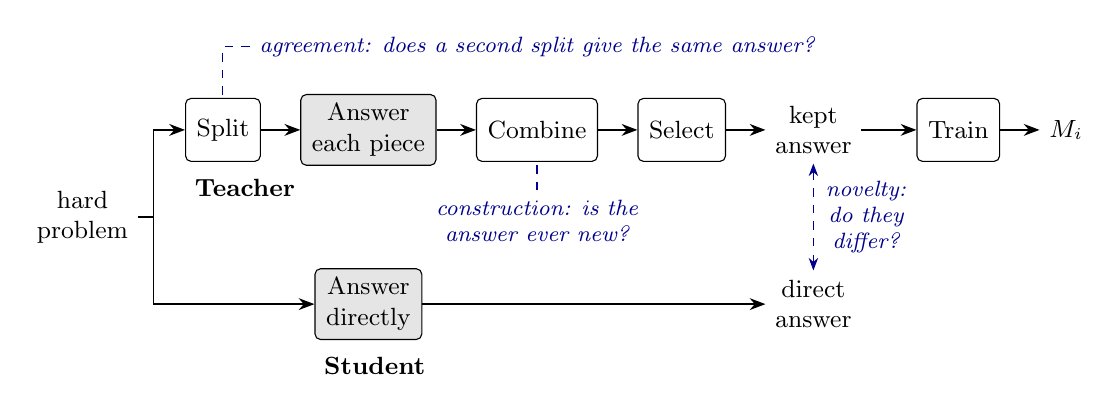
\begin{tikzpicture}[
  font=\small,
  node distance=5mm and 5mm,
  box/.style={draw, rounded corners=2pt, minimum height=8mm,
    inner xsep=4pt, align=center},
  model/.style={box, fill=black!10},
  plain/.style={align=center},
  flow/.style={-{Stealth[length=2mm]}, semithick},
  chk/.style={font=\footnotesize\itshape, text=blue!55!black, align=center},
  chkline/.style={dashed, blue!55!black},
]
% Teacher row
\node[box] (split) {Split};
\node[model, right=of split] (pieces) {Answer\\each piece};
\node[box, right=of pieces] (combine) {Combine};
\node[box, right=of combine] (select) {Select};
\node[plain, right=of select] (built) {kept\\answer};
\node[box, right=7mm of built] (train) {Train};
\node[plain, right=of train] (next) {$M_i$};
% Student row
\node[model, below=13mm of pieces] (direct) {Answer\\directly};
\node[plain] (dans) at (built |- direct) {direct\\answer};
% Problem
\node[plain, left=6mm of split] (x) at ($(split.west)!0.5!(split.west |-
  direct)$) {hard\\problem};
% Flows
\draw[flow] (x.east) -- ++(2mm,0) |- (split.west);
\draw[flow] (x.east) -- ++(2mm,0) |- (direct.west);
\draw[flow] (split) -- (pieces);
\draw[flow] (pieces) -- (combine);
\draw[flow] (combine) -- (select);
\draw[flow] (select) -- (built);
\draw[flow] (built) -- (train);
\draw[flow] (train) -- (next);
\draw[flow] (direct) -- (dans);
% Role labels
\node[plain, below=1mm of split.south west, anchor=north west]
  {\textbf{Teacher}};
\node[plain, below=1mm of direct.south west, anchor=north west]
  {\textbf{Student}};
% Checks
\draw[chkline, {Stealth[length=1.6mm]}-{Stealth[length=1.6mm]}]
  (built) -- node[chk, right=1pt] {novelty:\\do they\\differ?} (dans);
\node[chk, above=4mm of combine] (agr)
  {agreement: does a second split give the same answer?};
\draw[chkline] (agr.west) -| (split.north);
\node[chk] (con) at ($(combine.south)+(0,-7.5mm)$)
  {construction: is the\\answer ever new?};
\draw[chkline] (con.north) -- (combine.south);
\end{tikzpicture}
\caption{One round of self-improvement, seen as two roles of one model. Shaded
  boxes are calls to the model $M_{i-1}$. The teacher's kept answers are the
  training set $D_i$. Dashed lines mark where each check looks; none of them
  uses a correct answer to the hard problem.}
\label{fig:roles}
\end{figure}

\subsection{A worked example}
\label{sec:worked-example}

Figure~\ref{fig:example} walks through a concrete example of both roles in
action. Here, a model trained only on three- to seven-digit numbers is asked to
add two eight-digit numbers. Unsurprisingly, the student's direct attempt fails.
To solve it as a teacher, the model splits each number in two, adds the left
and right pieces separately, and concatenates the two results. With the first
split, this breaks down: the right-hand pieces sum to a five-digit number, and
the extra carry digit gets stuck awkwardly in the middle of the combined string
instead of carrying over to the left. However, the next two splits happen to
cut at boundaries with no carry, so both yield the right total.

What enters the training set next comes down to the selection rule. Without any
filtering, the teacher blindly keeps the flawed first answer. The filter
proposed by \citet{shin2026compositional}, which we call the \emph{no-carry
rule}, recognizes that an oversized partial sum signals an overflow error and
discards the example entirely. By contrast, our \emph{agreement rule} requires
no domain-specific arithmetic knowledge: it simply keeps an answer if at least
two different splits arrive at the same result.

\begin{figure}[t]
\centering
\small
\begin{tabular}{@{}lll@{}}
\toprule
\multicolumn{3}{@{}l}{\textbf{Problem:} \texttt{35128624 + 21415273}
  \quad (correct answer \texttt{56543897}, not available to the model)} \\
\midrule
\multicolumn{3}{@{}l}{\textbf{Student} answers directly:
  \texttt{56533897} \;$\times$} \\
\midrule
\multicolumn{3}{@{}l}{\textbf{Teacher} splits, answers each piece, and writes
  the sums side by side:} \\
Split & Sums of the pieces & Built answer \\
\texttt{3512|8624} & \texttt{3512+2141 = 5653},\;
  \texttt{8624+5273 = 13897} & \texttt{565313897} \;$\times$ \\
\texttt{351|28624} & \texttt{351+214 = 565},\;
  \texttt{28624+15273 = 43897} & \texttt{56543897} \;\checkmark \\
\texttt{35128|624} & \texttt{35128+21415 = 56543},\;
  \texttt{624+273 = 897} & \texttt{56543897} \;\checkmark \\
\midrule
\multicolumn{3}{@{}l}{\textbf{Selection} decides what is kept for training:} \\
No selection & keeps the first split's answer & \texttt{565313897}
  \;$\times$ \\
No-carry rule  & \texttt{13897} does not fit in four digits & nothing kept \\
Agreement rule & two of the three splits agree & \texttt{56543897}
  \;\checkmark \\
\bottomrule
\end{tabular}
\caption{One addition problem seen by the student and by the teacher. The
  marks \checkmark{} and $\times$ are for the reader: the model never sees
  them. The student's answer is illustrative. The no-carry rule is the
  hand-written filter of \citet{shin2026compositional}; the agreement rule
  needs no knowledge of carrying.}
\label{fig:example}
\end{figure}

\subsection{Two questions before every round}
\label{sec:two-questions}

Before committing to a training round, we draw a fresh batch of hard problems
and have the model play both roles. No weights are updated, and no correct
answers are consulted. Instead, we ask two diagnostic questions.

\paragraph{Is there anything new?} The \emph{novelty check} calculates the
fraction of the teacher's kept answers that actually differ from the student's
direct predictions. If nearly all of them match what the student already outputs,
training will be a dead end. With a reliable teacher, novelty is high on problem
lengths the student has yet to master, and drops near zero on lengths it
already knows. While comparing direct and decomposed answers has previously
been used to catch reasoning errors \citep{bottman2026operadic,yang2024decc}, we
use it here to gauge whether a training round has anything left to teach. Of
course, novelty alone cannot distinguish progress from regression: a different
answer might fix a student's mistake, or introduce a brand-new one.

\paragraph{Does a second split agree?} A valid solution should not depend on
where we happened to slice the input. Combining errors, on the other hand, are
usually sensitive to the cut point, as illustrated in Figure~\ref{fig:example} where a
carry ruins the first split while leaving the others untouched. To test for
this, the \emph{agreement check} re-derives each kept answer using alternative
splits and measures the fraction reproduced identically by at least one other
split, which we call the \emph{confirmed share}. A low confirmed share warns
that much of the teacher's training data is unreliable. Two caveats are worth
noting here. First, the alternative splits must cut at distinct positions; two
splits sharing a boundary will fail at that boundary in the exact same way,
giving a false sense of consensus. Second, agreement does not guarantee
correctness: two different splits can still converge on the same mistake.

The agreement rule of Figure~\ref{fig:example} is this same check, used as a
selection step. Because it keeps only answers that a second split confirms,
any teacher using it has a confirmed share of 100\% by construction, and only
the novelty check remains informative in that setting.

\subsection{One question per procedure}
\label{sec:one-question}

Our third diagnostic evaluates the decomposition procedure itself, not any
particular round, so it only needs to be run once per procedure.

\paragraph{Can the teacher build anything new?} The \emph{construction check}
measures how often the teacher's final answer is identical to one of the
individual sub-problem answers it started with. If this happens 100\% of the
time, the teacher is merely \emph{handing back} partial solutions: every answer
it produces for a hard problem is already something the model outputs for an
easier piece, so it can show the student nothing beyond the sub-problems.
Concatenating sums never falls into this trap, because the combined number is
always longer than either partial sum. On our second task, finding the longest
run of repeated characters in a string, the procedure from
\citet{shin2026compositional} always hands back: it simply returns the longest
run found inside an isolated piece, meaning it can never detect a run spanning
across a cut. Because this limitation is structural, we can measure it upfront
by substituting an oracle solver for the model before any training begins. In
practice, real models yielded identical scores on addition and nearly identical
ones on the string task (Table~\ref{tab:check3}).

That said, passing the construction check is necessary rather than sufficient.
A procedure might be capable of constructing novel answers in general while
still systematically filtering out the exact cases the student needs to see.
The no-carry rule illustrates this blind spot: it constructs valid multi-digit
sums beyond the student's reach, yet because it discards every problem
involving a carry across the boundary, the student is never shown a carry at
that position. The construction check is blind to this filtering bias, a
limitation whose consequences we examine in Section~\ref{sec:three-further-findings}.

\subsection{From answers to a prediction}
\label{sec:prediction}

For any given round and problem length, we combine our two per-round checks to
forecast one of three outcomes: the round will \emph{pay off}, \emph{do
nothing}, or \emph{do harm}. The rule also includes a third per-round check that we specified in advance:
because the teacher relies on the model's ability to solve smaller
sub-problems, a \emph{basics check} measures accuracy on easy problems.
The prediction is given by three questions asked in order
(Figure~\ref{fig:prediction}); the first that is answered ``no'' decides.

% Flowchart of the prediction rule. Needs in the preamble:
%   \usepackage{tikz}
%   \usetikzlibrary{arrows.meta,positioning}
\begin{figure}[t]
    \centering
    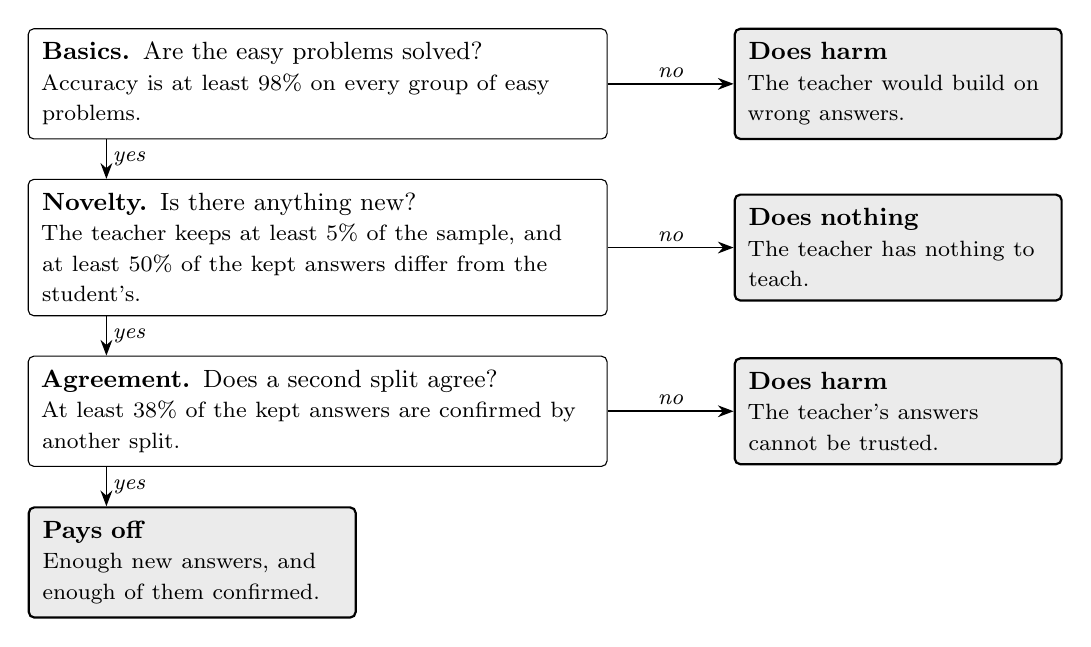
\begin{tikzpicture}[
      font=\small,
      every node/.append style={execute at begin node={\hyphenpenalty=10000\relax}},
      node distance=5mm and 16mm,
      q/.style={draw, rounded corners=2pt, text width=70mm, align=left,
        inner sep=5pt},
      res/.style={draw, thick, rounded corners=2pt, text width=38mm,
        align=left, inner sep=5pt, fill=black!8},
      flow/.style={-{Stealth[length=2mm]}, semithick},
      lab/.style={font=\footnotesize\itshape, inner sep=2pt},
    ]
    \node[q] (basics) {\textbf{Basics.} Are the easy problems solved?\\
      {\footnotesize Accuracy is at least 98\% on every group of easy problems.}};
    \node[q, below=of basics] (novelty) {\textbf{Novelty.} Is there anything
      new?\\
      {\footnotesize The teacher keeps at least 5\% of the sample, and at least
      50\% of the kept answers differ from the student's.}};
    \node[q, below=of novelty] (agree) {\textbf{Agreement.} Does a second split
      agree?\\
      {\footnotesize At least 38\% of the kept answers are confirmed by another
      split.}};
    \node[res, right=of basics] (harm1) {\textbf{Does harm}\\
      {\footnotesize The teacher would build on wrong answers.}};
    \node[res, right=of novelty] (nothing) {\textbf{Does nothing}\\
      {\footnotesize The teacher has nothing to teach.}};
    \node[res, right=of agree] (harm2) {\textbf{Does harm}\\
      {\footnotesize The teacher's answers cannot be trusted.}};
    \node[res, below=of agree.south west, anchor=north west] (pays)
      {\textbf{Pays off}\\
      {\footnotesize Enough new answers, and enough of them confirmed.}};
    \draw[flow] (basics) -- node[lab, above] {no} (harm1);
    \draw[flow] (novelty) -- node[lab, above] {no} (nothing);
    \draw[flow] (agree) -- node[lab, above] {no} (harm2);
    \draw[flow] ([xshift=10mm]basics.south west) --
      node[lab, right] {yes} ([xshift=10mm]novelty.north west);
    \draw[flow] ([xshift=10mm]novelty.south west) --
      node[lab, right] {yes} ([xshift=10mm]agree.north west);
    \draw[flow] ([xshift=10mm]agree.south west) --
      node[lab, right] {yes} ([xshift=10mm]pays.north west);
    \end{tikzpicture}
    \caption{How the checks give a prediction for one round at one problem length.
      The questions are asked in order, and the first ``no'' decides. Thresholds
      were calibrated on a separate set of pilot runs prior to evaluation (Section~\ref{sec:setup}).
      The basics check is the only one that uses correct answers, and only for easy problems.}
    \label{fig:prediction}
    \end{figure}

Novelty is tested before agreement because an answer the student already knows
can never change the model. Both the ordering of these rules and their numerical 
thresholds were calibrated on a separate set of pilot runs prior to evaluation (Section~\ref{sec:setup}).
The construction check is omitted from these round-by-round rules since it is
run once upfront to verify whether a procedure can ever teach anything beyond
the pieces.

Table~\ref{tab:checks} summarizes all four checks, and
Section~\ref{sec:do-the-checks-predict} evaluates how well our forecasts matched
actual training outcomes. In short, the novelty and agreement checks proved
highly predictive, whereas the basics check did not.

\begin{table}[t]
\centering
\caption{The checks. Kept answers are those the teacher's selection step
  retains for training. The first three use no correct answers. The version of
  the construction check for addition was defined after the evaluation runs.}
\label{tab:checks}
\small
\begin{tabular}{@{}l>{\raggedright\arraybackslash}p{0.25\linewidth}>{\raggedright\arraybackslash}p{0.36\linewidth}l@{}}
\toprule
Check & Question & What is measured & Asked \\
\midrule
Novelty & Is there anything new? & Share of kept answers that differ from the
  student's direct answer & Every round \\
\addlinespace
Agreement & Does a second split agree? & Share of kept answers that another
  split reproduces & Every round \\
\addlinespace
Construction & Can the teacher build anything new? & Share of the teacher's
  answers identical to an answer for one of the pieces & Once per procedure \\
\addlinespace
Basics & Are the easy problems solved? & Accuracy on easy problems & Every
  round \\
\bottomrule
\end{tabular}
\end{table}
\section{Single-round setup}
\label{sec:setup}

\paragraph{Model, task, and training.}
Following \citet{shin2026compositional}---a compositional variant of
self-training on a model's own outputs \citep{lee2025selfimproving}---we train
a character-level Transformer (approximately 14M parameters, no positional
encoding) from scratch to add two numbers of equal length. A starting model is
first trained with correct answers on sums of 3 to 7 digits, which we call
\emph{easy problems}. Four successive rounds then extend the maximum length to
9, 11, 13, and 15 digits. In each round, the teacher generates answers to fresh
problems at every length from 8 digits up to the current maximum until it has
kept 10,000 answers per length, and the model trains on these together with
easy problems that it answers itself. Sums are split into two pieces up to 12
digits and three at 13 to 15, so every piece has 3 to 7 digits. Each length
uses three fixed splits (five at 13 to 15 digits) with no shared cut positions;
the first supplies the candidate answer, and the others serve the agreement
check and the agreement rule.

\paragraph{Teachers.}
With the no-carry filter of \citet{shin2026compositional}, every addition round
in our reproduction paid off. Testing a three-way predictor requires rounds
that also stall or degrade the model, so we construct a benchmark spanning all
three outcomes by design. We run four teachers: the \emph{no-carry rule} and
\emph{agreement rule} (Section~\ref{sec:two-roles}), expected to help; \emph{no
selection}, which keeps the first split's answer unconditionally and thus
trains on every carry error; and \emph{sample and vote}, which does not split
at all, instead sampling five direct answers and keeping one that appears at
least three times \citep{wang2023selfconsistency}. Additional cases come from
starting models stopped early (weak piece accuracy), from applying \emph{no
selection} to a model previously trained with the no-carry rule (so accuracy
can fall from near 100\%), and from retraining lengths already learned in
earlier rounds.

\paragraph{Cases and outcomes.}
A \emph{case} is one combination of teacher, starting model, round, and problem
length. Before the round, the checks run on 2,000 fresh problems of that length
to issue a prediction; afterwards, the outcome is scored from held-out test
accuracy before and after training. At a length the model already knew, a
change within 3 points counts as \emph{did nothing}, and a larger drop---at
that length or on easy problems---counts as \emph{did harm}. At a new length,
accuracy starts near zero and cannot fall, nor does a rise alone show that the
right rule was learned, so we compare against the best accuracy achieved by any
teacher at that length in the same round and from the same starting model: a
rise of at least 20 points ending within 10 points of the best \emph{paid off};
a rise ending 30 points or more below the best taught wrong answers and counts
as \emph{did harm}; a rise under 10 points \emph{did nothing}. A few
intermediate cases (such as partially learned lengths that rise further) are
left unclassified by this rule and examined separately in
Section~\ref{sec:errors}.

\paragraph{Calibration and evaluation.}
We trained five starting models from distinct random seeds: two for the
calibration runs used to set the rule of Section~\ref{sec:rule}, and three held
out for evaluation. Before any evaluation run began, the prediction rule, the
outcome rule, and a pre-specified pass mark---at least 90\% accuracy overall,
with at least five cases each of \emph{did nothing} and \emph{did harm}---were
frozen in a tagged commit. The three evaluation models produce 270 cases, of
which the outcome rule classifies 258. Because not every analysis in this paper
was fixed at the same moment, Appendix~\ref{app:fixed-when} records when
each was specified (Table~\ref{tab:fixed-when}).

\section{Predicting a round}
\label{sec:do-the-checks-predict}

The three evaluation models yield \gpNovGainCases{} cases in total, of which
the outcome rule classifies \gpCases{}. We ask two questions of them. First,
does the frozen threshold rule predict what a single round will do before
training (Section~\ref{sec:main-result}), and what explains its errors
(Section~\ref{sec:errors})? Second, do Propositions~\ref{prop:novelty}
and~\ref{prop:agreement} hold quantitatively underneath the thresholds: does
novelty track the size of the gain (Section~\ref{sec:novelty-bound}), and does
split agreement isolate right answers without a task filter
(Section~\ref{sec:confirmed-right})?

\subsection{The main result}
\label{sec:main-result}
\label{sec:which-check}

Across the three held-out starting models, the prediction rule was correct in
\gpCorrect{} of \gpCases{} cases (\gpCorrectPct\%), compared with
\gpDidNothingPct\% for always predicting \emph{does nothing}, the most frequent
outcome (Table~\ref{tab:p9b-confusion}). Every prediction of \emph{pays off}
and of \emph{does nothing} was correct, all \gpHarmful{} harmful cases were
flagged as \emph{does harm}, and all nine errors were false alarms of harm,
meeting the pass mark set before evaluation. Broken down by starting model, the
rule was correct in \gpCorrectModelTwo{}, \gpCorrectModelThree{}, and
\gpCorrectModelFour{} of the \gpCasesModelTwo{} cases per seed.

% Generated by `uv run python -m gainpred.writeup`; do not edit by hand.
\begin{table}[t]
\centering
\caption{Predictions before training against outcomes after training, for the
  258 evaluation cases. Every error is a prediction of harm that did not occur.}
\label{tab:p9b-confusion}
\small
\begin{tabular}{lrrr}
\toprule
 & \multicolumn{3}{c}{Prediction} \\
\cmidrule(l){2-4}
Outcome & Pays off & Does nothing & Does harm \\
\midrule
Paid off & 31 & 0 & 6 \\
Did nothing & 0 & 175 & 3 \\
Did harm & 0 & 0 & 43 \\
\bottomrule
\end{tabular}
\end{table}


The \gpCases{} cases are not independent tests. They fall into eight kinds, and
within each kind the outcome is nearly always the same: what a round does is
largely determined by which teacher is used and whether the length is new
(Supplement, Table~\ref{S-tab:p9b-cases}). The checks are given neither piece
of information; they infer what the round will do from the model's answers
alone. The novelty check (including its 5\% retention floor) decided
\gpByNovelty{} cases, all correctly: lengths already learned, every round
taught by sample and vote, and rounds with no selection at lengths it had
already taught. Agreement decided \gpByAgreement{} cases, all correctly,
separating the teachers that paid off at new lengths from no selection, which
taught wrong answers there. The basics check decided the remaining
\gpByBasics{} cases and accounts for all nine errors. Each check falls into two
well-separated clusters with the threshold inside the gap between them
(Supplement, Figure~\ref{S-fig:checks}). Running the checks took
\gpChecksCostAdditionPct\% of a round's compute; starting the round and extrapolating
from its first 200 updates was less accurate, took \gpBaselineCostAdditionPct\% of a
round's compute, and required correct answers
(Supplement~\ref{S-app:prediction}).

\subsection{Novelty bounds the change}
\label{sec:novelty-bound}

The prediction rule uses novelty only as a cutoff, whereas
Proposition~\ref{prop:novelty} makes a quantitative statement: novelty bounds
the magnitude of the change a round can produce, and equals the gain when the
teacher is right. We tested this after all experiments on the same cases, with
no prediction recorded in advance. In \gpNovGainWithin{} of \gpNovGainCases{}
cases, test accuracy changed by no more than the novelty plus 3 points, the
margin allowed for a round that did nothing (Appendix~\ref{app:evidence},
Figure~\ref{fig:novelty-gain}). When the teacher is right, the proposition
predicts that novelty, pre-round student error, and accuracy gain coincide. On
fully trained starting models, the no-carry rule and the agreement rule are
right almost without exception: across their \gpNovGainSound{} cases, the gain
lay within 5 points of the novelty in \gpNovGainSoundChange{} (largest gap
\gpNovGainSoundChangeGap), including the \gpNovGainSoundBetween{} partially
learned cases where novelty sits away from 0\% and 100\% and all three numbers
move together. For a teacher known to be right, pre-round novelty is therefore
a direct forecast of the points a round will add. Without a check on teacher
accuracy, novelty remains only an upper bound: where sample and vote kept
answers, they mostly differed from the student's, yet accuracy never changed by
more than \gpNovGainVoteMax{} points.

\subsection{Confirmed answers are right}
\label{sec:confirmed-right}
\label{sec:agreement-filter}

Proposition~\ref{prop:agreement} requires $\varepsilon$ to be small for the
agreement check ($a_T \ge c - \varepsilon$) and small relative to $c$ for the
agreement rule ($1 - \varepsilon/c$), and $\varepsilon$ is the one quantity a
model cannot measure for itself. After all experiments finished, we measured it
with correct answers; before any answer was scored, we recorded one prediction
for each condition across the \gpTaFullCases{} split-based cases from fully
trained starting models: that $\varepsilon$ would be at most 2\% in every case,
and that at least 98\% of confirmed answers ($1 - \varepsilon/c$) would be
correct in every case. Both held. The largest $\varepsilon$ was
\gpTaPOneWorst\%, and the lowest accuracy among confirmed answers was
\gpTaPTwoWorst\% (Appendix~\ref{app:evidence},
Table~\ref{tab:teacher-accuracy}).

Agreement therefore identifies the right answers even of a teacher that is
mostly wrong. With no selection, the teacher was right on only
\gpTaNoSelectAccLow--\gpTaNoSelectAccHigh\% of its answers, yet at least
\gpTaNoSelectAccConfirmedLow\% of those confirmed by another split were
correct. This is why the agreement rule can replace a filter written for the
task: it encodes no knowledge of carrying, and after four rounds its student
was within \gpGapMean{} points of the no-carry student on average across 8 to
15 digits, at the price of taking \gpBuildRatio{} times as long to fill the
same training quota (Supplement~\ref{S-app:prediction}). The guarantee has a
limit. On weak starting models, which answer the pieces themselves poorly,
$\varepsilon$ reached \gpTaWeakWrongConfirmedHigh\% while $c$ also fell,
pulling confirmed accuracy down with it (Table~\ref{tab:teacher-accuracy}):
split agreement tests the composition step directly, and piece accuracy only
indirectly.


\subsection{Where the prediction was wrong}
\label{sec:errors}

All nine errors on classified cases come from the ten cases whose starting
model failed the basics check: the rule predicted harm in all ten and was right
once, because a model just below the 98\% pass mark still yields a teacher that
is mostly right. Without the basics check, the other two checks alone would
have been correct in \gpCorrectNoBasics{} of \gpCases{} cases
(\gpCorrectNoBasicsPct\%); we computed this afterwards, and the frozen rule
remains our main result.

The outcome rule leaves \gpNoOutcome{} further cases unclassified. In ten of
them, a length the model already answered correctly more than half the time
rose to 98\% or higher, while the rule predicted \emph{does nothing}. These are
errors in substance: all ten were taught by an accurate teacher, so novelty
equaled the student's remaining error, which lay below 50\% and was read by the
rule as nothing left to learn. The fault lies in the coarse 50\% cutoff rather
than in novelty itself, which came within \gpNovGainSoundChangeGap{} points of
the actual gain in every one of the ten cases. Counting all \gpNoOutcome{}
unclassified cases as errors gives \gpCorrectAllPct\%.

\paragraph{From single rounds to a loop.}
Taken together, these results separate the two quantities from the thresholds
wrapped around them. The frozen rule predicts single-round outcomes in
\gpCorrectPct\% of classified cases and flags every harmful round, and its
misses---false alarms from the 98\% basics floor and partially learned lengths
missed by the 50\% novelty cutoff---come from discretizing continuous signals
rather than from failures of the bounds themselves. Underneath those cutoffs,
split agreement isolates right answers ($\ge\gpTaPTwoWorst\%$ accurate on fully
trained models) even when an unfiltered teacher is mostly wrong, and novelty
forecasts the resulting gain within a few points whenever the teacher is right.
Those are the two pieces a multi-round loop needs: a task-free filter to keep
composition errors out of training, and a quantitative measure of whether
anything remains to be learned.

\section{A ladder from 8 to 39 digits}
\label{sec:ladder}

Section~\ref{sec:do-the-checks-predict} studied rounds one at a time. We now
ask what a model needs to keep teaching itself across many rounds, far beyond
its supervised starting range, without additional labels or a hand-written
filter. Four arms test this by adding one ingredient at a time from the same
starting models. The study is exploratory: we recorded no predictions in
advance, though all definitions and rules were fixed before any run with one
exception stated in Appendix~\ref{app:ladder}
(Appendix~\ref{app:fixed-when}).

\subsection{Design}
\label{sec:ladder-design}

\paragraph{One procedure from 8 to 39 digits.}
Each starting model is trained with correct answers on sums of 3 to 7 digits,
as in Section~\ref{sec:setup}. From there, 16 rounds each add two lengths, from
8 and 9 digits up to 38 and 39; four rounds form a \emph{stage} of eight
lengths. Every sum is split into two pieces at three positions adjacent to its
midpoint (for example, a 12-digit sum as $5+7$, $6+6$, and $7+5$), so every
piece is shorter than the lengths being taught. Up to 12 digits all pieces lie
in the supervised starting range; from 18 digits onward, every piece is a
length the model has taught itself. Beyond 7 digits, no correct answers and no
hand-written rules are used anywhere. In each round, the model first measures
the two quantities of Section~\ref{sec:teacher-and-student} on
\gpLadCheckSums{} fresh sums per new length, then builds \gpLadQuota{} training
answers per length, trains on them alongside the answers kept in earlier
rounds, and is evaluated at every length (Appendix~\ref{app:ladder}).

\paragraph{Four arms.}
The four arms differ only in how training answers are produced at each new
length.
\emph{Direct}: the model's direct answers to the new sums.
\emph{Composed}: the answer composed from the first split unconditionally.
\emph{Composed and agreed}: an answer produced by at least two of the three
splits, applying the agreement rule of Section~\ref{sec:two-roles}.
\emph{Self-paced}: as in \emph{Composed and agreed}, except that the model
builds a full training set for a length only if pre-round novelty there is at
least \gpLadThreshold\%. Otherwise it retains just the confirmed answers from
the \gpLadCheckSums{}-sum check sample so the length stays represented in
later rounds, and if neither new length reaches \gpLadThreshold\% it skips
training in that round altogether. The \gpLadThreshold\% cutoff was chosen on
the logs of an earlier loop before these runs
(Appendix~\ref{app:ladder}).

\paragraph{Starting models and stopping.}
We run three new starting models from unused random seeds. Within each seed,
all four arms start from the same checkpoint and draw the same sums. A stage
counts as \emph{learned} if test accuracy is at least \gpLadLearnedLevel\% at
every one of its eight lengths after its fourth round; an arm stops after the
first stage it fails to learn.

\subsection{What each ingredient adds}
\label{sec:ladder-result}

\begin{table}[t]
\centering
\caption{The four arms on three starting models: stages learned, of four,
  and lowest accuracy (\%) at any length taught, after the arm's last round
  (8 to 15 digits for the first two arms, 8 to 39 for the others).}
\label{tab:ladder}
\small
\begin{tabular}{@{}lcccccc@{}}
\toprule
 & \multicolumn{2}{c}{Seed 5} & \multicolumn{2}{c}{Seed 6} &
   \multicolumn{2}{c}{Seed 7} \\
\cmidrule(lr){2-3}\cmidrule(lr){4-5}\cmidrule(l){6-7}
The model trains on & Stages & Lowest & Stages & Lowest & Stages & Lowest \\
\midrule
Its direct answers & \gpLadArmOneSeedFiveStages & \gpLadArmOneSeedFiveLowest &
  \gpLadArmOneSeedSixStages & \gpLadArmOneSeedSixLowest &
  \gpLadArmOneSeedSevenStages & \gpLadArmOneSeedSevenLowest \\
Composed answers, unfiltered & \gpLadArmTwoSeedFiveStages & \gpLadArmTwoSeedFiveLowest &
  \gpLadArmTwoSeedSixStages & \gpLadArmTwoSeedSixLowest &
  \gpLadArmTwoSeedSevenStages & \gpLadArmTwoSeedSevenLowest \\
Composed and agreed answers & \gpLadArmThreeSeedFiveStages &
  \gpLadArmThreeSeedFiveLowest & \gpLadArmThreeSeedSixStages &
  \gpLadArmThreeSeedSixLowest & \gpLadArmThreeSeedSevenStages &
  \gpLadArmThreeSeedSevenLowest \\
The same, self-paced & \gpLadArmFourSeedFiveStages &
  \gpLadArmFourSeedFiveLowest & \gpLadArmFourSeedSixStages &
  \gpLadArmFourSeedSixLowest & \gpLadArmFourSeedSevenStages &
  \gpLadArmFourSeedSevenLowest \\
\bottomrule
\end{tabular}
\end{table}

\paragraph{Direct answers and unfiltered composition fail.}
Trained on its direct answers, the model learned no stage on any seed
(Table~\ref{tab:ladder}): it answered at most \gpLadArmOneEightHigh\% of
8-digit sums and \gpLadArmOneLongerHigh\% of longer ones. Trained on
unfiltered compositions it learned no stage either, and its failure is exact.
Only \gpLadArmTwoKeptRightLow--\gpLadArmTwoKeptRightHigh\% of its training
answers were right, namely those with no carry across the split. After
stage~1 it answered \gpLadArmTwoCarryHigh\% of test sums with such a carry at
every length, against
\gpLadArmTwoNoCarryShortLow--\gpLadArmTwoNoCarryShortHigh\% of the others at 8
to 12 digits. From 13 digits the first split contains a piece the model taught
itself with the same error, and accuracy on sums without a carry halves to
\gpLadArmTwoNoCarryLongLow--\gpLadArmTwoNoCarryLongHigh\%
(Appendix~\ref{app:ladder}, Figure~\ref{fig:ladder}): it learned the
composition, error included.

\paragraph{Split agreement carries the model to 39 digits.}
Keeping only answers on which two splits agree, the model learned all four
stages on all three seeds, with a lowest final accuracy of
\gpLadArmThreeSeedFiveLowest, \gpLadArmThreeSeedSixLowest, and
\gpLadArmThreeSeedSevenLowest\% across 8 to 39 digits. The share of its kept
answers that were right never fell below \gpLadArmThreeSeedFiveKeptRightLow\%
on any seed. On seed~5 two rounds diverged and were repeated under a rule added
after the first (Appendix~\ref{app:ladder}). Given correct answers only up to
7 digits and no rule about carrying, the model taught itself to add 39-digit
numbers.

\subsection{The model paces itself}
\label{sec:ladder-pace}

\begin{figure}[t]
\centering
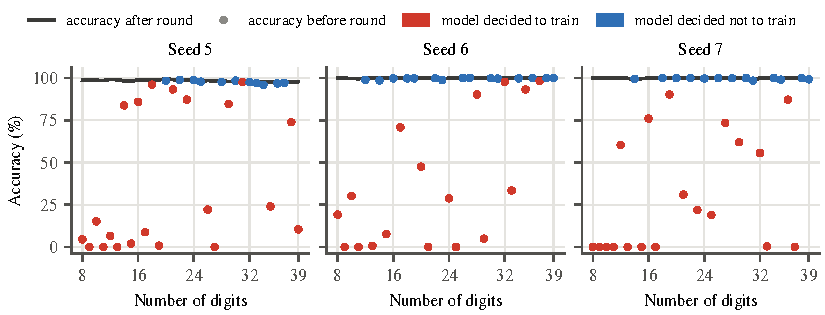
\includegraphics[width=\linewidth]{generated/figure_ladder_decisions.pdf}
\caption{The self-paced arm's decisions. Each circle is one length: the
  accuracy of the model's direct answers just before the round that would
  teach it, red where the model then trained and blue where it did not. The
  line is the accuracy after that round.}
\label{fig:ladder-decisions}
\end{figure}


In the fourth arm the model decides before each round, without correct
answers, where it still has something to learn.
Figure~\ref{fig:ladder-decisions} sets each decision beside the model's
actual accuracy, which it never sees: where it decided not to train, it
already stood where it would end up; where it decided to train, there was a
gap, and training closed it. The arm
learned all four stages on all three seeds while skipping
\gpLadSkippedSeedFive, \gpLadSkippedSeedSix, and \gpLadSkippedSeedSeven{} of
the 32 lengths. It used \gpLadUpdatesShareSeedFive,
\gpLadUpdatesShareSeedSix, and \gpLadUpdatesShareSeedSeven\% of the third
arm's training updates and \gpLadGpuShareSeedFive, \gpLadGpuShareSeedSix,
and \gpLadGpuShareSeedSeven\% of its GPU time, and its final accuracy over 8
to 39 digits differed from the third arm's by $\gpLadDiffMeanSeedFive$,
$\gpLadDiffMeanSeedSix$, and $\gpLadDiffMeanSeedSeven$ points
(Appendix~\ref{app:ladder}, Table~\ref{tab:ladder-pace}). At every skipped length it already answered at
least \gpLadSkippedDirectLowest\% of sums directly, and none fell below
\gpLadSkippedLaterLowest\% in any later round; at the \gpLadWouldSkip{}
lengths where the rule would have skipped in the third arm, building raised
accuracy by only $\gpLadWouldSkipGainMean$ points on average. As in
Section~\ref{sec:novelty-bound}, novelty worked as a quantity: over the
\gpLadNoveltyGapCases{} lengths of the third arm it differed from the gain
the round then produced by \gpLadNoveltyGapMedian{} points at the median and
\gpLadNoveltyGapHigh{} at most.

\section{Discussion}
\label{sec:discussion-and-limits}

\paragraph{What the results say.}
In the setting we studied, a model can tell from its own answers what a round
of self-improvement will do, select its own training data, and decide where to
train. Two quantities carry all three roles: \emph{novelty} (how often the
teacher's answers differ from the student's) and the \emph{confirmed share}
(how often a second split reproduces them), standing in for the correct answers
and hand-written filter used by \citet{shin2026compositional}. As a filter,
agreement between splits is what lets the loop work at all: without it, the
model learns nothing from direct answers or learns the composition's carry
error. As a measurement, novelty tracks how much of each length remains to be
learned closely enough to skip a third to a half of the work at no cost in
accuracy---provided any cutoff placed on it matches the question asked
(flagging a large single-round jump versus checking whether any gap remains).
We stopped the ladder at 39 digits by choice: on two starting models, final
accuracy at the longest sums matched that at the shortest, while on the third
errors accumulated slowly, leaving open how much further it would have climbed.

\paragraph{Relation to other work.}
\label{sec:related}
Training a model on outputs produced with an auxiliary procedure---tree search
\citep{anthony2017thinking}, decomposition \citep{christiano2018amplification},
or richer prompts \citep{zhang2026basersi}---is standard practice, though
training on self-generated outputs can also degrade a model
\citep{shumailov2024collapse}. Whereas prior work uses the teacher--student gap
to drive training, or predicts self-training gains from dataset statistics
\citep{vanasch2016predicting}, we use that gap before training to decide
whether and where to train. Two concurrent studies ask related questions with
stronger signals: \citet{li2026evolve} select self-distillation data using
gradients and ground-truth labels, and \citet{he2026recursive} filter agent
generations only after training and measuring their gain; we decide beforehand
from outputs alone. For estimating accuracy without labels, prior work relies
on agreement across models \citep{baek2022agreement}, across two views in
co-training \citep{blum1998cotraining}, or among a model's own samples at test
time \citep{wang2023selfconsistency} and during self-training
\citep{shafayat2025selftrain}. Our sample-and-vote baseline follows the last
approach and taught nothing; agreement across distinct splits acts instead like
two views inside a single model, informative precisely because the computation
paths and their errors differ. Finally, on length generalization, removing
positional encodings \citep{kazemnejad2023positional} or adding position-aware
embeddings \citep{mcleish2024abacus} extends addition
architecturally---\citet{zhou2024algorithms} characterize which algorithms
extrapolate in this way---while filtered self-training on direct answers
extends our architecture one digit at a time \citep{lee2025selfimproving}; here
the architecture stays fixed and split-confirmed composition carries it across
32 lengths.

\paragraph{Scope and outlook.}
\label{sec:limits}
Our empirical evidence is of two kinds: the single-round predictor was frozen
before evaluation, whereas the 39-digit ladder is exploratory---its rules were
fixed before running, save for the divergence retry rule added on the first
seed, and its pacing threshold was set from logs of an earlier loop. Using one
small model, three evaluation seeds, and a synthetic task was a deliberate
choice so every output could be scored exactly and harmful rounds induced
cleanly. Extending the same two quantities to larger models and open-ended
tasks will test three assumptions built into our setup. First, the checks
evaluate a supplied procedure that admits distinct splits; they do not discover
how to decompose a task. Second, they inspect only the answers a teacher keeps,
not what selection omits: a teacher that is right on every answer it keeps
can still harm the student by leaving a whole class of problems out of
training, and neither quantity would show it. Third, exact
string match will need to give way to semantic agreement where valid answers
are not unique.

\paragraph{Use of AI.}
Large language models and coding assistants were used to write experiment and
plotting code, orchestrate runs, aggregate and tabulate logs into tables and
figures, consolidate the appendices and supplement, and edit prose. All
hypotheses, experimental designs, code, and numerical results were verified by
the author, who takes full responsibility for the contents of this paper.



\bibliographystyle{plainnat}
\bibliography{refs}

\begin{appendices}
% Appendix: only what is needed to check the claims of the main text.
% Everything else is in supplement.tex (built to supplement.pdf).

\noindent The appendices contain what is needed to check the claims of the
main text. Further tables and settings are in the
supplementary material that follows them; references of the form S1 or
Table~S1 are to that supplement. The code, the frozen protocol and the logs
of every run are at \repourl.

\section{What was fixed when}
\label{app:fixed-when}

The evidential weight of a result depends on
when it was fixed, and Table~\ref{tab:fixed-when} classifies our results
accordingly. The prediction of single rounds belongs to the first row.
Results in the third row carried a prediction or a threshold that was
recorded in the repository before the corresponding numbers were computed.
The ladder is in the fourth row: its rules were recorded before any of its
code was written, but no outcome was predicted. Results in the last row are
observations made on data we had already seen, experiments designed while
they ran, or rules added after seeing a result. Every run we launched, including those that failed,
is documented in the repository.

\begin{table}[htbp]
\centering
\caption{What was fixed when. Each result is reported in the section given.}
\label{tab:fixed-when}
\small
\begin{tabular}{@{}>{\raggedright\arraybackslash}p{0.3\linewidth}>{\raggedright\arraybackslash}p{0.66\linewidth}@{}}
\toprule
Status & Results \\
\midrule
Fixed before the evaluation runs & The prediction rule and its thresholds; the
  outcome rule; the success criterion (Section~\ref{sec:main-result}) \\
\addlinespace
Planned before the evaluation runs, with no pass mark & The agreement rule
  against the no-carry rule (Section~\ref{sec:confirmed-right}) \\
\addlinespace
Defined after the evaluation runs, and fixed before its own results were
  computed & How often confirmed answers are right
  (Section~\ref{sec:confirmed-right}); the thresholds of the baseline
  (Supplement~\ref{S-app:prediction}) \\
\addlinespace
Rules fixed before any run, with no outcome predicted & The ladder
  (Section~\ref{sec:ladder}): its four arms, the splits, what counts as a
  stage learned, when an arm stops, the threshold of the self-paced arm
  (chosen on the logs of an earlier loop; Appendix~\ref{app:ladder}), the
  three random seeds and their order \\
\addlinespace
Computed afterwards, designed while running, or added after seeing a result
  & Novelty against the size of the change
  (Sections~\ref{sec:novelty-bound} and~\ref{sec:ladder-pace}); the result
  without the basics check (Section~\ref{sec:errors}); the rule for
  repeating a diverged round, written after the first such round on seed~5
  and in place before seeds 6 and~7 (Appendix~\ref{app:ladder});
  the margins of the checks and the variant of the baseline
  (Supplement~\ref{S-app:prediction}) \\
\bottomrule
\end{tabular}
\end{table}


\section{Evidence for Section~\ref{sec:do-the-checks-predict}}
\label{app:evidence}

Figure~\ref{fig:novelty-gain} plots the change in accuracy against novelty
for every evaluation case (Section~\ref{sec:novelty-bound}), and
Table~\ref{tab:teacher-accuracy} gives the accuracy of the teachers' kept
answers (Section~\ref{sec:confirmed-right}).

\begin{figure}[htbp]
\centering
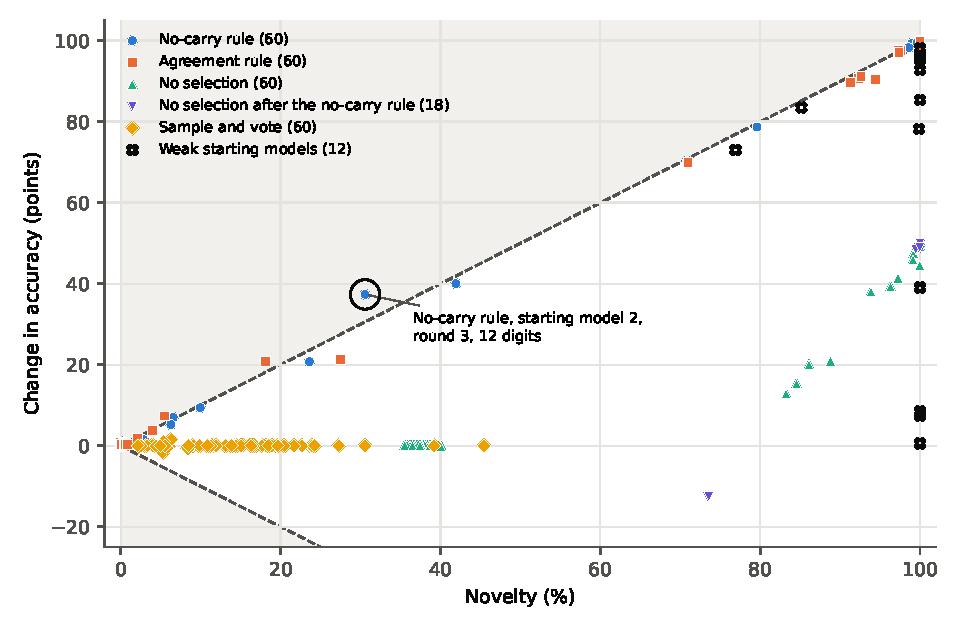
\includegraphics[width=\linewidth]{generated/figure_novelty_gain.pdf}
\caption{Change in accuracy against novelty, one point per evaluation case
  (all \gpNovGainCases, with or without an outcome). Novelty is measured on
  the teacher's kept answers before the round; the change is the accuracy on
  the test problems of that length after the round minus before. Dashed
  lines mark a change equal to plus or minus the novelty, the bound of
  Proposition~\ref{prop:novelty}; points in the shaded area lie outside it.
  The circled case is the only one more than 3 points outside.}
\label{fig:novelty-gain}
\end{figure}

% Built from the macros of generated/numbers.tex (same cells as
% generated/table_teacher_accuracy.tex, without the Cases column).
\begin{table}[htbp]
\centering
\caption{Accuracy of the teachers' kept answers in the evaluation runs,
  measured against the correct sums after all experiments. Each cell is the
  range over cases, in \% of a case's kept answers. The first four rows are
  the \gpTaFullCases{} cases from fully trained starting models. ``Wrong
  but confirmed'' is $\varepsilon$ of Proposition~\ref{prop:agreement}.}
\label{tab:teacher-accuracy}
\small
\begin{tabular}{@{}lcccc@{}}
\toprule
 & Teacher & Confirmed & Wrong but & Accuracy among \\
Teacher & accuracy & share & confirmed & confirmed \\
\midrule
No-carry rule & \gpTaNoCarryAccLow--\gpTaNoCarryAccHigh &
  \gpTaNoCarryConfirmedLow--\gpTaNoCarryConfirmedHigh
  & \gpTaNoCarryWrongConfirmedLow--\gpTaNoCarryWrongConfirmedHigh &
  \gpTaNoCarryAccConfirmedLow--\gpTaNoCarryAccConfirmedHigh \\
Agreement rule & \gpTaAgreementAccLow--\gpTaAgreementAccHigh &
  \gpTaAgreementConfirmedLow
  & \gpTaAgreementWrongConfirmedLow--\gpTaAgreementWrongConfirmedHigh &
  \gpTaAgreementAccConfirmedLow--\gpTaAgreementAccConfirmedHigh \\
No selection & \gpTaNoSelectAccLow--\gpTaNoSelectAccHigh &
  \gpTaNoSelectConfirmedLow--\gpTaNoSelectConfirmedHigh
  & \gpTaNoSelectWrongConfirmedLow--\gpTaNoSelectWrongConfirmedHigh &
  \gpTaNoSelectAccConfirmedLow--\gpTaNoSelectAccConfirmedHigh \\
No selection after the no-carry rule
  & \gpTaNoSelectAfterAccLow--\gpTaNoSelectAfterAccHigh &
  \gpTaNoSelectAfterConfirmedLow--\gpTaNoSelectAfterConfirmedHigh
  & \gpTaNoSelectAfterWrongConfirmedLow--\gpTaNoSelectAfterWrongConfirmedHigh &
  \gpTaNoSelectAfterAccConfirmedLow--\gpTaNoSelectAfterAccConfirmedHigh \\
\midrule
Weak starting models & \gpTaWeakAccLow--\gpTaWeakAccHigh &
  \gpTaWeakConfirmedLow--\gpTaWeakConfirmedHigh
  & \gpTaWeakWrongConfirmedLow--\gpTaWeakWrongConfirmedHigh &
  \gpTaWeakAccConfirmedLow--\gpTaWeakAccConfirmedHigh \\
\bottomrule
\end{tabular}
\end{table}

\section{Details of the ladder}
\label{app:ladder}

\noindent The code and the logs call a split a \emph{cut}.

\paragraph{Splits.} A sum of $n$ digits is split so that the left piece has
$h-1$, $h$ and $h+1$ digits, where $h$ is $n/2$ rounded down. Every piece has
at least 3 digits and is shorter than both lengths its round adds. Up to 12
digits all pieces have at most 7 digits; from 13 digits some split has a
piece of 8 digits or more; from 18 digits every piece of every split has. The
longest piece has 21 digits (Supplement~\ref{S-app:ladder-more},
Table~\ref{S-tab:ladder-splits}). Sums are drawn so that no piece begins with
the digit 0.

\paragraph{One round.} (i) \emph{Measure.} On \gpLadCheckSums{} fresh sums per
new length the model answers directly and through each of the three splits.
From these we log the direct accuracy, the share of sums on which two splits
agree, the confirmed share of the first split's answers, and novelty. Over
all rounds of the third arm the first split's answer was right for
\gpLadCutOneRightLow--\gpLadCutOneRightHigh\% of sums, the confirmed share was
\gpLadConfirmedShareLow--\gpLadConfirmedShareHigh\%, and two splits agreed on
\gpLadAgreedShareLow--\gpLadAgreedShareHigh\%. (ii) \emph{Build.} Fresh sums
are drawn until \gpLadQuota{} answers are kept for each new length, or
\gpLadDrawCapFactor{} times as many sums have been drawn. (iii) \emph{Train}
on the new answers, all answers kept in earlier rounds, and
\gpLadReplayPerLength{} sums at each length from 3 to 7 that the model answers
itself, for \gpLadPasses{} passes over this set and at least \gpLadMinUpdates{}
updates, with the settings of Section~\ref{sec:setup}. (iv) \emph{Test} on
\gpLadTestPerGroup{} held-out sums with a carry across the first split and
\gpLadTestPerGroup{} without, at every length taught so far.

\paragraph{The self-paced arm.} Novelty is the share of the sums on which two
splits agree whose agreed answer differs from the direct answer. A length is
built if novelty is at least \gpLadThreshold\%, or if fewer than
\gpLadMinAgreed{} of the \gpLadCheckSums{} sums have two splits that agree,
since then the teacher, not the student, is the problem. For a length that
is not built, the agreed answers of the measurement are stored and repeated
to the weight of a built length; the number of updates is computed from the
unrepeated examples. The gain of a round at a length is the accuracy on
the test sums after the round minus the direct
accuracy in the measurement before it. Across the three seeds, the highest
novelty at a skipped length was \gpLadSkippedNoveltyHighSeedFive,
\gpLadSkippedNoveltyHighSeedSix{} and \gpLadSkippedNoveltyHighSeedSeven\%.
The \gpLadThreshold\% threshold was chosen before these runs, on the logs of
an earlier loop over 16 to 39 digits. That loop started from a model taught 8
to 15 digits with the no-carry rule and trained on every length whatever its
checks said. It is documented with its logs in the repository, as are further
experiments not reported here.

\begin{table}[htbp]
\centering
\caption{The self-paced arm against the arm that builds answers at every
  length. Shares are the self-paced arm's as a percentage of the other's.
  The difference is in final accuracy, in points, averaged over the lengths
  8 to 39.}
\label{tab:ladder-pace}
\small
\begin{tabular}{@{}lccc@{}}
\toprule
 & Seed 5 & Seed 6 & Seed 7 \\
\midrule
Lengths skipped, of 32 & \gpLadSkippedSeedFive & \gpLadSkippedSeedSix &
  \gpLadSkippedSeedSeven \\
Rounds without training, of 16 & \gpLadRoundsSkippedSeedFive &
  \gpLadRoundsSkippedSeedSix & \gpLadRoundsSkippedSeedSeven \\
Training updates (\%) & \gpLadUpdatesShareSeedFive &
  \gpLadUpdatesShareSeedSix & \gpLadUpdatesShareSeedSeven \\
GPU time (\%) & \gpLadGpuShareSeedFive & \gpLadGpuShareSeedSix &
  \gpLadGpuShareSeedSeven \\
Difference in accuracy (points) & $\gpLadDiffMeanSeedFive$ &
  $\gpLadDiffMeanSeedSix$ & $\gpLadDiffMeanSeedSeven$ \\
Lowest accuracy at a skipped length (\%) & \gpLadSkippedFinalLowSeedFive &
  \gpLadSkippedFinalLowSeedSix & \gpLadSkippedFinalLowSeedSeven \\
\bottomrule
\end{tabular}
\end{table}

\paragraph{Diverged rounds.} A round after which accuracy is below
\gpLadDivergedLevel\% at any length from 3 to 7 digits is trained once
more, from the same weights and on the same examples, with a different batch
order; a second failure ends the arm. This rule was written after the first
such round, in the third arm on seed~5, and that arm was continued under it;
seeds 6 and~7 ran with it from the start. It was triggered
\gpLadDivergedEvents{} times, both in the third arm on seed~5,
and \gpLadDivergedRedosFailed{} of the repeated rounds diverged again. The
arm's first run, which stopped after the first diverged round under the
rules then in force, is reported with the others in the repository.

\begin{figure}[htbp]
\centering
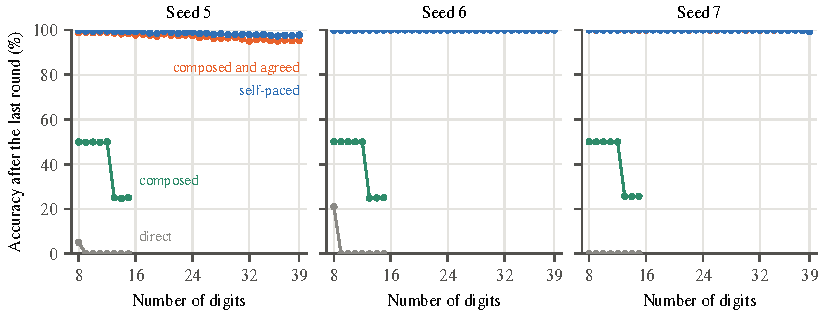
\includegraphics[width=\linewidth]{generated/figure_ladder_accuracy.pdf}
\caption{Accuracy at each length after an arm's last round, for the three
  starting models. The first two arms stopped after stage~1 (8 to 15
  digits).}
\label{fig:ladder}
\end{figure}

\paragraph{Cost.} The three seeds cost \$\gpLadCostSeedFive,
\$\gpLadCostSeedSix{} and \$\gpLadCostSeedSeven{} of GPU time.

\end{appendices}

% ---- Supplementary material, in the same PDF ----
\clearpage
\makeatletter
% Inside the supplement, a label foo is stored as S-foo, so that the main
% text's \ref{S-foo} finds it. A \ref{foo} inside the supplement uses S-foo
% if it exists and otherwise the main text's foo.
\let\gp@label\label
\let\gp@ref\ref
\renewcommand{\label}[1]{\gp@label{S-#1}}
\renewcommand{\ref}[1]{\@ifundefined{r@S-#1}{\gp@ref{#1}}{\gp@ref{S-#1}}}
\makeatother
\setcounter{section}{0}
\setcounter{table}{0}
\setcounter{figure}{0}
\renewcommand{\thesection}{S\arabic{section}}
\renewcommand{\thetable}{S\arabic{table}}
\renewcommand{\thefigure}{S\arabic{figure}}
\renewcommand{\theHsection}{S\arabic{section}}   % distinct link targets
\renewcommand{\theHtable}{S\arabic{table}}
\renewcommand{\theHfigure}{S\arabic{figure}}

\begin{center}
  {\Large\bfseries Supplementary Material}
\end{center}

\noindent Section, table and figure numbers that begin with S are in this
supplement; all others refer to the paper. Every table and figure here is
generated from the logs in the repository (\repourl), which also holds the
code, the frozen protocol with its amendments, and a record of every run.

\section{Details of the setup}
\label{app:setup-details}
\label{app:settings}

\paragraph{Outcomes.} Table~\ref{tab:outcomes} states the outcome rule of
Section~\ref{sec:setup}. Its boundaries suit the present setting, in which a
successful round takes a new length from zero to 70\% or more at once and an
unsuccessful one leaves it near zero; elsewhere they would have to be chosen
anew.

\begin{table}[htbp]
\centering
\caption{The outcome of a round at one problem length. Scores are accuracies
  on test problems, in percentage points. ``The best'' is the highest score
  any teacher's student reached at that length, in the same round and from the
  same starting model.}
\label{tab:outcomes}
\small
\begin{tabular}{@{}lll@{}}
\toprule
Length & Outcome & Condition \\
\midrule
Could already do & Did nothing & Changes by at most 3 points \\
 & Did harm & Falls by more than 3 points, here or on easy problems \\
\addlinespace
New & Paid off & Rises by at least 20 points, to within 10 of the best \\
 & Taught wrong answers & Rises, but ends 30 points or more below the best \\
 & \quad (counted as harm) & \\
 & Did little or nothing & Rises by less than 10 points \\
\bottomrule
\end{tabular}
\end{table}


\paragraph{Adjustments before the freeze.}
Four adjustments were made between the calibration runs and the freeze.
First, we placed novelty ahead of agreement, which raised the number of
correctly predicted calibration cases from 107 to 166 of 176. Second, we
increased the number of splits for 13- to 15-digit problems from three to
five, because three splits artificially depressed the confirmed share of an
otherwise sound teacher. Third, we added the 10-point and 50\% conditions to
the outcome rule. Fourth, we added the requirement that at least 5\% of
answers be kept, which guards against sampling noise: when a teacher keeps
fewer than a hundred answers, the proportion of new ones varies widely
between samples.


\paragraph{Reproduction.}
Table~\ref{tab:reproduction} compares our accuracies with those reported by
\citet{shin2026compositional}. The two are not directly comparable: they
train for eight rounds and test up to 23 digits, whereas we train for four
and test up to 15. Within those limits the pattern is the same. With their
filter the model reaches nearly full accuracy at every length it has been
taught, and without it accuracy remains far lower.

% Generated by `uv run python -m gainpred.writeup`; do not edit by hand.
\begin{table}[H]
\centering
\caption{Accuracy (\%) on the reproduction test set: 100 problems per length, 3
  to 15 digits, greedy answers, scored after all experiments on the saved models
  of the evaluation runs (mean of three runs, range in brackets). Shin et al.'s
  figures are those they report (their Table 10 and appendix C.1); they train 8
  rounds up to 23 digits and test up to 23 digits, so their columns cover 8-23
  and 23 digits, ours 8-15 and 15 digits. The no-carry rule corresponds to their
  filtered composition, no selection to their unfiltered composition.}
\label{tab:reproduction}
\small
\begin{tabular}{lrr}
\toprule
Model & Mean over new lengths & Longest length \\
\midrule
This paper (8--15 digits; 15 digits) &  &  \\
Starting model & 1.8 (0.4--3.5) & 0.0 (0.0--0.0) \\
No-carry rule, round 1 & 31.5 (27.0--37.1) & 0.0 (0.0--0.0) \\
No-carry rule, round 2 & 59.5 (56.8--61.3) & 0.0 (0.0--0.0) \\
No-carry rule, round 3 & 84.5 (84.2--85.0) & 0.0 (0.0--0.0) \\
No-carry rule, round 4 & 99.6 (98.9--100.0) & 99.0 (98.0--100.0) \\
No selection, round 1 & 10.8 (10.5--11.0) & 0.0 (0.0--0.0) \\
No selection, round 2 & 25.2 (24.8--26.2) & 0.0 (0.0--0.0) \\
No selection, round 3 & 40.8 (39.0--41.9) & 0.0 (0.0--0.0) \\
No selection, round 4 & 41.8 (36.0--44.9) & 24.0 (17.0--28.0) \\
\midrule
Shin et al. (8--23 digits; 23 digits) &  &  \\
Starting model & 0.0 & 0.0 \\
Filtered composition, last round (8) & 93.7 & 80.0 \\
Unfiltered composition, last round (8) & 33.5 & 11.0 \\
\bottomrule
\end{tabular}
\end{table}



\section{Further results on the predictions}
\label{app:prediction}

This section contains the material referred to in
Section~\ref{sec:do-the-checks-predict} of the paper: the kinds of case
(Table~\ref{tab:p9b-cases}), the margins of the checks
(Figure~\ref{fig:checks}), the cases from weak starting models
(Table~\ref{tab:weak}), the cases without an outcome
(Table~\ref{tab:no-outcome}), the comparison with training briefly
(Tables~\ref{tab:baseline} and~\ref{tab:cost-addition}), and the agreement
rule against the no-carry rule
(Figure~\ref{fig:exp1}).

% Generated by `uv run python -m gainpred.writeup`; do not edit by hand.
\begin{table}[t]
\centering
\caption{Cases correctly predicted, by kind of case, in the evaluation runs.}
\label{tab:p9b-cases}
\small
\begin{tabular}{lrr}
\toprule
Kind of case & Cases & Correctly predicted \\
\midrule
Agreement rule, new lengths & 14 & 14 \\
No-carry rule, new lengths & 14 & 14 \\
No selection & 60 & 60 \\
Sample and vote & 60 & 60 \\
Lengths already learned & 79 & 79 \\
Starting model stopped early (weak) & 10 & 1 \\
New length started midway & 3 & 3 \\
No selection after the no-carry rule (run f) & 18 & 18 \\
\bottomrule
\end{tabular}
\end{table}


\paragraph{Margins.}
Figure~\ref{fig:checks} shows why these predictions are robust. The values of
each check form two clusters, and the threshold lies in the gap between them.
Leaving aside the cases decided by the 5\% minimum, novelty was at most
\gpNoveltyMarginLow\% wherever the prediction was ``does nothing'' and at
least \gpNoveltyMarginHigh\% everywhere else. The confirmed share was at most
\gpConfirmedMarginLow\% in the \gpConfirmedHarmCases{} cases it predicted to
do harm, and at least \gpConfirmedMarginHigh\% in the \gpConfirmedPaysCases{}
it predicted to pay off. Any thresholds within these ranges yield the same
predictions. We computed the ranges after the evaluation runs; the
thresholds themselves were fixed beforehand.

% Generated by `uv run python -m gainpred.writeup`; do not edit by hand.
\begin{figure}[htbp]
\centering
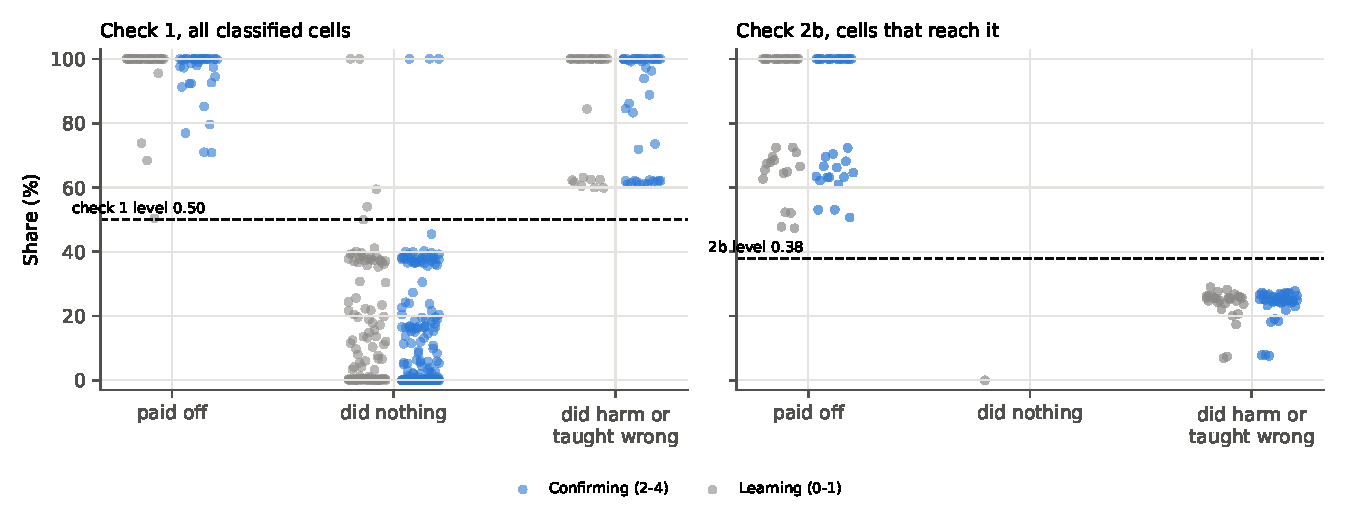
\includegraphics[width=\linewidth]{generated/figure_checks.pdf}
\caption{Novelty (all cases with an outcome) and confirmed share (cases that
  reach the agreement check) by outcome. Dashed: the levels fixed before the
  evaluation runs. Shaded: the range within which a level gives the same
  predictions on the evaluation runs (computed after them).}
\label{fig:checks}
\end{figure}


\paragraph{The basics check.} Ten cases with an outcome come from starting
models that fail the basics check, so the rule predicted harm in all ten. It
was right once (Table~\ref{tab:weak}). Three of
these models were just below the pass mark, with at least 91\% on every size
of easy problem. All six of their cases paid off, as they do for a fully
trained starting model. The other three failed some sizes of easy problem
almost entirely. Their rounds mostly did little, and taught wrong answers in
one case. Weak basics therefore did not predict harm in our runs.

The measurements of Section~\ref{sec:confirmed-right} explain why. A model
just below the pass mark still yields a teacher that is mostly right, and its
rounds pay off. A much weaker model yields a teacher whose accuracy varies
sharply from one length to the next, from \gpTaWeakAccLow\% to
\gpTaWeakAccHigh\%, and its confirmed share fell with that accuracy, to
\gpTaWeakConfirmedLow\%. What the basics check was intended to establish, the
agreement check establishes more directly, on the hard problems themselves.
Without the basics check, the two other checks would have been correct in
\gpCorrectNoBasics{} of \gpCases{} cases (\gpCorrectNoBasicsPct\%). We
computed this after the evaluation runs, and the rule as frozen remains our
main result.

One of the remaining errors is a failure of imitation
(Section~\ref{sec:what-changes}). At 8 digits, one of the very weak models
yielded a teacher that was right on nearly all of its kept answers, and the
student's accuracy nevertheless rose by less than 10 points. A teacher can be
right and the student unable to follow.

% Generated by `uv run python -m gainpred.writeup`; do not edit by hand.
\begin{table}[htbp]
\centering
\caption{The 12 cases from weak starting models (stopped early), evaluation
  runs, including those without an outcome. Easy: lowest accuracy (\%) over easy
  sizes 3-7 before the round (the basics check needs 98\% at every size).
  Before, after: accuracy (\%) at that length; best: the best teacher's after,
  same starting model and round.}
\label{tab:weak}
\small
\resizebox{\linewidth}{!}{%
\begin{tabular}{lrrrrrlll}
\toprule
Starting model & Easy & Length & Before & After & Best & Outcome & Prediction
  & Without basics \\
\midrule
2 (1,425 updates) & 4.7 & 8 & 0.2 & 85.5 & 100.0 & without an outcome
  & does harm & pays off \\
2 (1,425 updates) & 4.7 & 9 & 0.0 & 39.0 & 100.0 & taught wrong answers
  & does harm & does harm \\
2 (2,200 updates) & 91.8 & 8 & 14.9 & 98.3 & 100.0 & paid off & does harm
  & pays off \\
2 (2,200 updates) & 91.8 & 9 & 0.0 & 96.2 & 100.0 & paid off & does harm
  & pays off \\
3 (3,450 updates) & 97.8 & 8 & 0.0 & 98.0 & 99.8 & paid off & does harm
  & pays off \\
3 (3,450 updates) & 97.8 & 9 & 0.0 & 95.3 & 100.0 & paid off & does harm
  & pays off \\
3 (3,500 updates) & 0.3 & 8 & 0.0 & 8.5 & 99.8 & did nothing & does harm
  & pays off \\
3 (3,500 updates) & 0.3 & 9 & 0.0 & 0.6 & 100.0 & did nothing & does harm
  & does harm \\
4 (2,250 updates) & 96.1 & 8 & 24.1 & 97.0 & 99.2 & paid off & does harm
  & pays off \\
4 (2,250 updates) & 96.1 & 9 & 0.0 & 92.8 & 98.3 & paid off & does harm
  & pays off \\
4 (3,000 updates) & 0.9 & 8 & 0.2 & 78.4 & 99.2 & without an outcome & does harm
  & pays off \\
4 (3,000 updates) & 0.9 & 9 & 0.0 & 7.4 & 98.3 & did nothing & does harm
  & does harm \\
\bottomrule
\end{tabular}
}
\end{table}

% Generated by `uv run python -m gainpred.writeup`; do not edit by hand.
\begin{table}[H]
\centering
\caption{The 12 evaluation cases without an outcome, and the gap in the outcome
  rule each falls in. Before, after: accuracy (\%) at that length; novelty in
  \%.}
\label{tab:no-outcome}
\small
\resizebox{\linewidth}{!}{%
\begin{tabular}{llrrrrrll}
\toprule
Teacher & Starting model & Round & Length & Before & After & Novelty
  & Prediction & Gap in the outcome rule \\
\midrule
Agreement rule & 2 & 2 & 10 & 78.6 & 99.8 & 27.5 & does nothing
  & started above 50\%, rose more than 3 points \\
Agreement rule & 3 & 2 & 10 & 79.2 & 99.8 & 18.1 & does nothing
  & started above 50\%, rose more than 3 points \\
Agreement rule & 3 & 3 & 12 & 96.2 & 100.0 & 3.9 & does nothing
  & started above 50\%, rose more than 3 points \\
Agreement rule & 4 & 2 & 10 & 91.1 & 98.5 & 5.4 & does nothing
  & started above 50\%, rose more than 3 points \\
No-carry rule & 2 (weak) & 1 & 8 & 0.2 & 85.5 & 100.0 & does harm
  & rose 20 points or more, 10-30 below the best \\
No-carry rule & 2 & 3 & 12 & 62.6 & 100.0 & 30.6 & does nothing
  & started above 50\%, rose more than 3 points \\
No-carry rule & 2 & 4 & 14 & 93.0 & 100.0 & 6.6 & does nothing
  & started above 50\%, rose more than 3 points \\
No-carry rule & 3 & 3 & 12 & 79.2 & 100.0 & 23.6 & does nothing
  & started above 50\%, rose more than 3 points \\
No-carry rule & 3 & 4 & 14 & 90.6 & 100.0 & 10.0 & does nothing
  & started above 50\%, rose more than 3 points \\
No-carry rule & 4 (weak) & 1 & 8 & 0.2 & 78.4 & 99.9 & does harm
  & rose 20 points or more, 10-30 below the best \\
No-carry rule & 4 & 2 & 10 & 58.3 & 98.4 & 41.9 & does nothing
  & started above 50\%, rose more than 3 points \\
No-carry rule & 4 & 4 & 14 & 93.5 & 98.8 & 6.3 & does nothing
  & started above 50\%, rose more than 3 points \\
\bottomrule
\end{tabular}
}
\end{table}


\paragraph{Compared with training briefly.}
\label{sec:vs-baseline}
\label{sec:baselines}
We compare the prediction rule with two baselines. The first always predicts
the most frequent outcome. The second is the obvious alternative to checks:
start the round, train for 200 of the 3,000 updates, measure accuracy on the
test set, and extrapolate from the early change. We defined this baseline
after the evaluation runs; its thresholds were tuned on the calibration runs
and recorded before any of its results on the evaluation runs were read.
Unlike our checks, it requires correct answers to the hard problems.

Computational cost is measured as wall-clock time on a single GPU. For each
round, we compare the time needed to run the checks with the total time of
the round, that is, generating the kept answers and training on them.

The obvious alternative is to start the round and inspect it
. As originally run, this baseline was correct
in \gpBaselineCorrect{} of \gpCases{} cases (\gpBaselineCorrectPct\%). A
variant that we defined after the evaluation runs, in the baseline's favor,
reached \gpVariantCorrect{} (\gpVariantCorrectPct\%), still below the checks
(Table~\ref{tab:baseline}). The baseline missed harmful cases: it flagged
\gpBaselineHarmFlagged{} of \gpHarmful{}, and the variant
\gpVariantHarmFlagged{}, whereas the checks flagged all \gpHarmful{}. It
outperformed the checks on the \gpWeakCases{} cases from weak starting
models, with \gpBaselineWeakCorrect{} and \gpVariantWeakCorrect{} correct
against \gpOursWeakCorrect{}, because it does not rely on the basics check.

% Generated by `uv run python -m gainpred.writeup`; do not edit by hand.
\begin{table}[t]
\centering
\caption{Cells matched by our checks (before training, no reference answers) and by the baseline (200 updates, then accuracy on the test problems, which needs their reference answers), confirming runs. Baseline levels fitted on starting points 0-1: G = 15, H = 47, D = 51. Cost per round: checks 9\%, baseline 56\% of a full round.}
\label{tab:baseline}
\small
\begin{tabular}{lrrr}
\toprule
 & Cells & Our checks & Baseline \\
\midrule
All cells & 258 & 249 & 224 \\
Paid off & 37 & 31 & 32 \\
Did nothing & 178 & 175 & 154 \\
Did harm or taught wrong answers & 43 & 43 & 38 \\
Agreement rule, new lengths & 14 & 14 & 14 \\
No-carry rule, new lengths & 14 & 14 & 12 \\
No selection & 60 & 60 & 55 \\
Sample and vote & 60 & 60 & 39 \\
Lengths already learned & 79 & 79 & 79 \\
Starting model stopped early (weak) & 10 & 1 & 4 \\
New length started midway & 3 & 3 & 3 \\
No selection after the no-carry rule (run f) & 18 & 18 & 18 \\
\bottomrule
\end{tabular}
\end{table}


The baseline is also more expensive and more demanding. It took
\gpBaselineCostAdditionPct\% of the computing time of a round, because it must first
build the round's training answers, and it requires correct answers to the
hard problems. The checks took \gpChecksCostAdditionPct\%
(Table~\ref{tab:cost-addition}) and require none. Rounds are short in this
setting, so these proportions would differ with longer training: the cost of
the checks depends on the number of problems examined, not on the length of
training.

% Generated by `uv run python -m gainpred.writeup`; do not edit by hand.
\begin{table}[htbp]
\centering
\caption{Seconds per round on one A10 GPU, evaluation runs on addition: whole
  round (build, replay, checks, 3,000 updates; evaluation not timed) and the
  checks alone.}
\label{tab:cost-addition}
\small
\begin{tabular}{lrrrr}
\toprule
Teacher & Rounds & Round s & Checks s & Checks \% \\
\midrule
No-carry rule & 12 & 309 & 34 & 11 \\
Agreement rule & 12 & 573 & 49 & 9 \\
No selection & 12 & 282 & 34 & 12 \\
Sample and vote & 12 & 932 & 52 & 6 \\
No selection after the no-carry rule & 3 & 310 & 40 & 13 \\
No-carry rule, weak starting models & 6 & 195 & 10 & 5 \\
\bottomrule
\end{tabular}
\end{table}


\paragraph{Agreement against the hand-written filter.}
\label{sec:agreement-vs-filter}

The agreement rule keeps an answer whenever two splits produce it, and
encodes no knowledge of carrying. After four rounds, the resulting student
was on average within \gpGapMean{} percentage points of the student trained
with the no-carry rule at every length from 8 to 15 digits
(Figure~\ref{fig:exp1}; Table~\ref{tab:passmark}), and trailed it by at most \gpGapWorst{} points in
the worst single run. Even on problems with a carry across the first split,
the largest gaps were \gpGapMeanCarry{} points on average and
\gpGapWorstCarry{} points in the worst run. We had not specified in advance
how closely the two had to match.

% Generated by `uv run python -m gainpred.writeup`; do not edit by hand.
\begin{figure}[htbp]
\centering
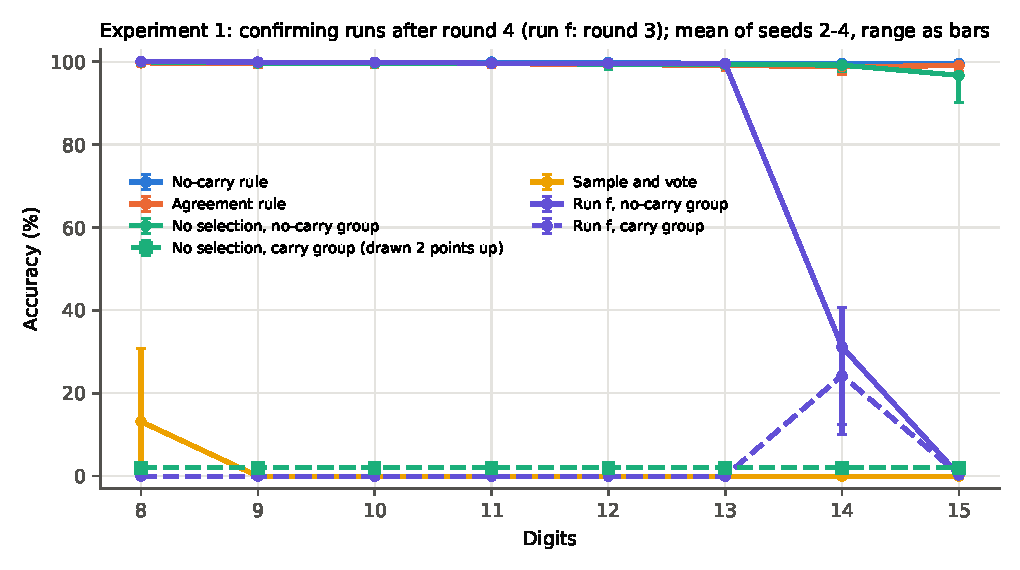
\includegraphics[width=\linewidth]{generated/figure_exp1.pdf}
\caption{Accuracy after round 4 (no selection after the no-carry rule: after its
  one round, round 3), evaluation runs; mean over the three starting models,
  range as bars.}
\label{fig:exp1}
\end{figure}


The measurements of Section~\ref{sec:confirmed-right} explain how this is
possible. Agreement does not require a teacher that is usually right. With no
selection, the first split's answer was correct in only
\gpTaNoSelectAccLow--\gpTaNoSelectAccHigh\% of cases, yet the answers that
another split confirmed were correct in at least
\gpTaNoSelectAccConfirmedLow\%. The agreement rule keeps such answers and
discards the rest, and its kept answers were correct in at least
\gpTaAgreementAccLow\% of cases. A filter written for the task encodes why an
answer is wrong. Agreement relies only on wrong answers not recurring from
one split to the next, which on this task was sufficient.

Dispensing with a hand-written filter has a cost. Because the agreement rule
must construct each answer several times, it took \gpBuildRatio{} times as
long as the no-carry rule to fill the same training quota. It also yields a
skewed sample: whereas roughly \gpNaturalCarryLow\% of fresh problems have a
carry at the first split, only \gpKeptAgreementLow\% to
\gpKeptAgreementHigh\% of the answers kept by the agreement rule do. Splits
are most likely
to agree when none of them errs, which removes the hardest cases
disproportionately. Finally, the rule presupposes a second valid way of
splitting the problem.

\citet{shin2026compositional} leave open how a composition procedure can be
validated without a task-specific filter. For addition, agreement across
splits provides one practical answer.

% Generated by `uv run python -m gainpred.writeup`; do not edit by hand.
\begin{table}[htbp]
\centering
\caption{Agreement rule minus no-carry rule after round 4, points, evaluation
  runs: mean over three starting models and worst single run (its starting
  model).}
\label{tab:passmark}
\small
\begin{tabular}{lrrrr}
\toprule
Digits & Mean gap & Worst run & Mean gap, carry & Worst run, carry \\
\midrule
8 & -0.2 & -0.5 (4) & -0.4 & -0.9 (4) \\
9 & -0.3 & -0.7 (4) & -0.4 & -1.1 (4) \\
10 & -0.3 & -0.8 (4) & -0.5 & -1.4 (4) \\
11 & -0.4 & -1.1 (4) & -0.5 & -1.3 (4) \\
12 & -0.5 & -1.3 (4) & -0.8 & -2.2 (4) \\
13 & -0.5 & -1.0 (4) & -1.0 & -1.8 (4) \\
14 & -0.8 & -1.8 (4) & -1.3 & -3.1 (4) \\
15 & -0.5 & -1.2 (4) & -1.1 & -2.2 (4) \\
\bottomrule
\end{tabular}
\end{table}


\section{The ladder: further details}
\label{app:ladder-more}

This section supplements Section~\ref{sec:ladder} of the paper.
Table~\ref{tab:ladder-splits} lists the three splits of every length.
Table~\ref{tab:ladder-lengths} gives, for every length and seed, the final
accuracy of the arm that builds answers everywhere and of the self-paced
arm, with the novelty the self-paced arm measured and what it then did.

% Generated by `uv run python -m gainpred.ladder_paper`; do not edit by hand.
\begin{table}[htbp]
\centering
\caption{The three splits of every length 8--39, each written as left piece +
  right piece (digits).}
\label{tab:ladder-splits}
\small
\setlength{\tabcolsep}{3pt}
\begin{tabular}{rlll@{\hspace{1.5em}}rlll}
\toprule
\multicolumn{4}{c}{8--23 digits} & \multicolumn{4}{c}{24--39 digits} \\
\cmidrule(lr){1-4}\cmidrule(lr){5-8}
Digits & Split 1 & Split 2 & Split 3 & Digits & Split 1 & Split 2 & Split 3 \\
\midrule
8 & 3 + 5 & 4 + 4 & 5 + 3 & 24 & 11 + 13 & 12 + 12 & 13 + 11 \\
9 & 3 + 6 & 4 + 5 & 5 + 4 & 25 & 11 + 14 & 12 + 13 & 13 + 12 \\
10 & 4 + 6 & 5 + 5 & 6 + 4 & 26 & 12 + 14 & 13 + 13 & 14 + 12 \\
11 & 4 + 7 & 5 + 6 & 6 + 5 & 27 & 12 + 15 & 13 + 14 & 14 + 13 \\
12 & 5 + 7 & 6 + 6 & 7 + 5 & 28 & 13 + 15 & 14 + 14 & 15 + 13 \\
13 & 5 + 8 & 6 + 7 & 7 + 6 & 29 & 13 + 16 & 14 + 15 & 15 + 14 \\
14 & 6 + 8 & 7 + 7 & 8 + 6 & 30 & 14 + 16 & 15 + 15 & 16 + 14 \\
15 & 6 + 9 & 7 + 8 & 8 + 7 & 31 & 14 + 17 & 15 + 16 & 16 + 15 \\
\midrule
16 & 7 + 9 & 8 + 8 & 9 + 7 & 32 & 15 + 17 & 16 + 16 & 17 + 15 \\
17 & 7 + 10 & 8 + 9 & 9 + 8 & 33 & 15 + 18 & 16 + 17 & 17 + 16 \\
18 & 8 + 10 & 9 + 9 & 10 + 8 & 34 & 16 + 18 & 17 + 17 & 18 + 16 \\
19 & 8 + 11 & 9 + 10 & 10 + 9 & 35 & 16 + 19 & 17 + 18 & 18 + 17 \\
20 & 9 + 11 & 10 + 10 & 11 + 9 & 36 & 17 + 19 & 18 + 18 & 19 + 17 \\
21 & 9 + 12 & 10 + 11 & 11 + 10 & 37 & 17 + 20 & 18 + 19 & 19 + 18 \\
22 & 10 + 12 & 11 + 11 & 12 + 10 & 38 & 18 + 20 & 19 + 19 & 20 + 18 \\
23 & 10 + 13 & 11 + 12 & 12 + 11 & 39 & 18 + 21 & 19 + 20 & 20 + 19 \\
\bottomrule
\end{tabular}
\end{table}

% Generated by `uv run python -m gainpred.ladder_paper`; do not edit by hand.
\begin{table}[htbp]
\centering
\caption{For each length and seed: final accuracy (\%) of the third arm (Agreed)
  and of the self-paced arm (Paced) after their last round, the self-paced arm's
  novelty in its check before the length's round (\% of pair-agreed answers that
  differ from the direct answer), and whether it built or skipped the length.}
\label{tab:ladder-lengths}
\scriptsize
\setlength{\tabcolsep}{3pt}
\begin{tabular}{rrrrlrrrlrrrl}
\toprule
 & \multicolumn{4}{c}{Seed 5} & \multicolumn{4}{c}{Seed 6}
 & \multicolumn{4}{c}{Seed 7} \\
\cmidrule(lr){2-5}\cmidrule(lr){6-9}\cmidrule(lr){10-13}
Digits & Agreed & Paced & Novelty & Paced did & Agreed & Paced & Novelty
  & Paced did & Agreed & Paced & Novelty & Paced did \\
\midrule
8 & 98.8 & 99.7 & 96.5 & built & 100.0 & 100.0 & 82.5 & built & 100.0 & 100.0
  & 100.0 & built \\
9 & 99.0 & 99.6 & 100.0 & built & 100.0 & 100.0 & 100.0 & built & 99.9 & 100.0
  & 100.0 & built \\
10 & 98.8 & 99.4 & 85.8 & built & 100.0 & 100.0 & 72.5 & built & 100.0 & 100.0
  & 100.0 & built \\
11 & 98.8 & 99.6 & 100.0 & built & 100.0 & 99.9 & 100.0 & built & 100.0 & 100.0
  & 100.0 & built \\
12 & 99.0 & 99.6 & 92.8 & built & 100.0 & 100.0 & 0.57 & skipped & 100.0 & 100.0
  & 40.6 & built \\
13 & 98.6 & 99.2 & 100.0 & built & 100.0 & 100.0 & 99.0 & built & 100.0 & 100.0
  & 100.0 & built \\
14 & 98.2 & 99.3 & 15.3 & built & 100.0 & 99.9 & 1.3 & skipped & 100.0 & 100.0
  & 0.15 & skipped \\
15 & 98.3 & 99.3 & 97.7 & built & 100.0 & 100.0 & 92.8 & built & 100.0 & 100.0
  & 100.0 & built \\
\midrule
16 & 97.8 & 99.2 & 12.4 & built & 100.0 & 100.0 & 0.00 & skipped & 100.0 & 100.0
  & 23.5 & built \\
17 & 98.1 & 99.4 & 89.1 & built & 100.0 & 100.0 & 28.5 & built & 100.0 & 100.0
  & 100.0 & built \\
18 & 97.6 & 98.6 & 2.9 & built & 100.0 & 100.0 & 0.15 & skipped & 100.0 & 100.0
  & 0.00 & skipped \\
19 & 97.1 & 98.4 & 99.4 & built & 100.0 & 100.0 & 0.15 & skipped & 100.0 & 100.0
  & 12.2 & built \\
20 & 98.2 & 99.5 & 0.29 & skipped & 100.0 & 100.0 & 51.8 & built & 100.0 & 100.0
  & 0.00 & skipped \\
21 & 97.6 & 99.0 & 4.9 & built & 100.0 & 100.0 & 100.0 & built & 99.9 & 100.0
  & 69.5 & built \\
22 & 97.4 & 98.5 & 0.30 & skipped & 100.0 & 99.9 & 0.00 & skipped & 99.9 & 100.0
  & 0.00 & skipped \\
23 & 97.8 & 98.8 & 12.7 & built & 100.0 & 100.0 & 1.4 & skipped & 100.0 & 100.0
  & 73.6 & built \\
\midrule
24 & 97.5 & 99.0 & 0.00 & skipped & 100.0 & 100.0 & 71.1 & built & 100.0 & 100.0
  & 0.15 & skipped \\
25 & 96.7 & 98.4 & 0.75 & skipped & 100.0 & 100.0 & 100.0 & built & 99.9 & 100.0
  & 79.3 & built \\
26 & 97.0 & 98.6 & 77.8 & built & 99.9 & 100.0 & 0.00 & skipped & 99.9 & 100.0
  & 0.14 & skipped \\
27 & 96.2 & 98.0 & 100.0 & built & 100.0 & 100.0 & 0.14 & skipped & 100.0
  & 100.0 & 24.4 & built \\
28 & 96.2 & 98.4 & 0.60 & skipped & 99.9 & 99.9 & 9.6 & built & 100.0 & 99.8
  & 0.00 & skipped \\
29 & 96.4 & 97.9 & 12.1 & built & 100.0 & 100.0 & 94.3 & built & 100.0 & 100.0
  & 32.7 & built \\
30 & 96.6 & 98.0 & 0.44 & skipped & 100.0 & 100.0 & 0.14 & skipped & 99.8
  & 100.0 & 0.00 & skipped \\
31 & 96.0 & 98.0 & 2.5 & built & 100.0 & 100.0 & 0.43 & skipped & 100.0 & 100.0
  & 1.3 & skipped \\
\midrule
32 & 95.0 & 97.9 & 0.30 & skipped & 100.0 & 100.0 & 2.3 & built & 99.9 & 100.0
  & 42.2 & built \\
33 & 95.7 & 97.8 & 1.3 & skipped & 100.0 & 100.0 & 66.1 & built & 99.9 & 100.0
  & 99.4 & built \\
34 & 96.0 & 98.0 & 1.2 & skipped & 100.0 & 100.0 & 0.59 & skipped & 100.0
  & 100.0 & 0.00 & skipped \\
35 & 95.2 & 97.6 & 75.1 & built & 99.9 & 100.0 & 7.1 & built & 100.0 & 100.0
  & 0.71 & skipped \\
36 & 95.0 & 97.3 & 1.2 & skipped & 99.9 & 100.0 & 0.00 & skipped & 99.9 & 99.9
  & 11.4 & built \\
37 & 95.5 & 97.7 & 1.7 & skipped & 99.9 & 100.0 & 2.4 & built & 100.0 & 100.0
  & 100.0 & built \\
38 & 95.2 & 97.5 & 21.7 & built & 99.9 & 100.0 & 0.00 & skipped & 100.0 & 99.8
  & 0.00 & skipped \\
39 & 95.2 & 97.8 & 89.0 & built & 100.0 & 100.0 & 0.14 & skipped & 100.0 & 99.4
  & 0.30 & skipped \\
\bottomrule
\end{tabular}
\end{table}


\paragraph{Training within a round.} Figure~\ref{fig:ladder-loss} shows the
training loss and the gradient norm during round~8, the round that adds 22
and 23 digits, for the run that diverged, its repetition, the self-paced arm
on the same seed, and the third arm on the two other seeds. In every run the
loss moves between about 0.01 and 1 and the gradient norm stays far above
the clipping level for the first two thirds of the round, while the learning
rate is constant; the loss falls only once the learning rate decays. The run
that diverged took one more such jump as the decay began and did not
recover.

\begin{figure}[htbp]
\centering
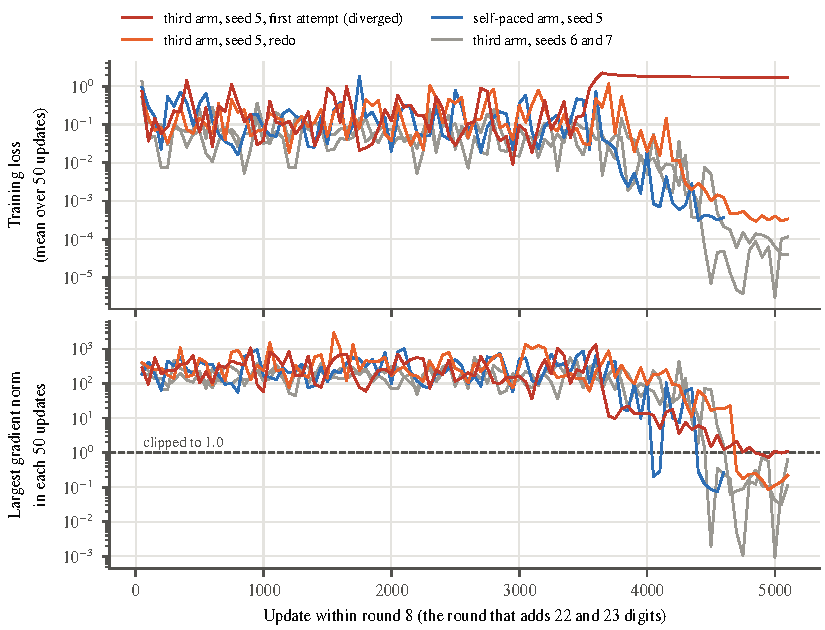
\includegraphics[width=\linewidth]{generated/figure_ladder_loss.pdf}
\caption{Training loss (top) and largest gradient norm before clipping
  (bottom) during round~8 of the ladder, per 50 updates.}
\label{fig:ladder-loss}
\end{figure}



\end{document}
